%% Light curves and demographics of tidal disruptions in self-sustaining
%% black hole engines.  Draft started 2026 September 05.
%% Items marked \colr{...} are TODOs.  Numbers quoted in the text are read
%% from products/results_fiducial.json (scripts/postprocess.py).
\documentclass[twocolumn,pdftex]{aastex701}
\usepackage{amsmath,amstext,amssymb}
\usepackage{xspace}
\usepackage{booktabs}
\hypersetup{colorlinks,citecolor=blue,linkcolor=magenta,urlcolor=blue}

\newcommand{\colr}[1]{{\bf \textcolor{red}{[#1]}}}
\newcommand{\msun}{M_{\odot}\xspace}
\newcommand{\mhsix}{M_{\rm h,6}\xspace}
\newcommand{\Sim}{\sim\!}
\newcommand{\mosfit}{{\tt MOSFiT}\xspace}
\newcommand{\gameq}{\Gamma_{\rm eq}\xspace}
\newcommand{\fom}{f_{\Omega}\xspace}
\newcommand{\rb}{r_{\rm b}\xspace}
\newcommand{\Av}{A_{V}\xspace}
\newcommand{\um}{\mu{\rm m}\xspace}
\newcommand{\lsst}{{\it Rubin}\xspace}
\newcommand{\wise}{{\it WISE}\xspace}
\newcommand{\neowise}{{\it NEOWISE}\xspace}
\newcommand{\jwst}{{\it JWST}\xspace}
\newcommand{\romantel}{{\it Roman}\xspace}
\newcommand{\euclid}{{\it Euclid}\xspace}
\newcommand{\spherex}{{\it SPHEREx}\xspace}
\newcommand{\fspark}{f_{\rm spark}\xspace}
\newcommand{\lamc}{\lambda_{\rm c}\xspace}

\shorttitle{Light Curves of Tidal Disruption Engines}
\shortauthors{Guillochon et al.}

% one wide float per page, allowed to take most of it, so figures ship on the page after their reference
\setcounter{dbltopnumber}{1}
\renewcommand{\dbltopfraction}{0.9}
\renewcommand{\dblfloatpagefraction}{0.8}

\begin{document}

\title{Light Curves and Demographics of Tidal Disruptions in Self-Sustaining Black Hole Engines}

\correspondingauthor{James Guillochon}

\author[0000-0002-9809-8215]{James Guillochon}
\affiliation{Independent Researcher}
\email[show]{guillochon@gmail.com}

\author{Friends}
\affiliation{To be determined}
\email{tbd@example.org}
%% placeholder for co-authors who have not yet agreed to join

\begin{abstract}
Tidal disruption events (TDEs) favor post-starburst hosts, and a self-sustaining ``engine'' has been proposed to explain the excess: the unbound debris of each disruption compresses the circumnuclear molecular clouds, the clouds compress the stellar cusp, and the cusp disrupts stars faster (Guillochon \& Loeb 2026). The equilibrium fixes the environment of every disruption: a black hole mass window of $7\times10^{5}$--$5\times10^{6}\,M_{\odot}$, a loss cone that is full at the sphere of influence, a stellar population $10^{8}$--$10^{9}$~yr old, and a molecular disk at $\sim5$~pc covering a fifth of the sky at $A_V\gtrsim50$. We compute the light curves such a population would produce with a population synthesis over hosts, stellar masses, and impact parameters, generating every light curve with MOSFiT, retaining the partial disruptions that dominate both populations, and setting the circularization time from the encounter geometry, which slows most flares in this mass range tenfold. With black holes that grow at 5\% of Eddington through the post-starburst phase and a disk resupplied by the host, a fifth of post-starburst nuclei host an active engine, the engine supplies the post-starburst share of the observed TDE rate for a rate normalization within a factor of 2--3 of fiducial, and the disruptions pile up at the floor with a median of $10^{6.1}\,M_{\odot}$. Engine flares peak $\sim100$~d after disruption, decline over $\sim300$~d, and reach $L\simeq10^{44}$~erg~s$^{-1}$ only for the quarter that are full disruptions; the partial majority is 1--2 dex fainter and fills the luminosity function to $M_g=-10$. A fraction 0.22 of events is obscured, as a step in inclination. The disk reprocesses each flare into a decade-long $10^{41}$--$10^{42}$~erg~s$^{-1}$, $\sim200$~K dust component at 15--30~$\mu$m, not a mid-infrared flare. We tabulate yields for Rubin, ZTF, Euclid, Roman, and SPHEREx.
\end{abstract}

\keywords{Tidal disruption (1696) --- Supermassive black holes (1663) --- Post-starburst galaxies (2176) --- Transient sources (1851) --- Interstellar dust extinction (837)}

\section{Introduction}\label{sec:intro}

Tidal disruption events (TDEs) are over-represented in post-starburst and quiescent Balmer-strong galaxies by one to two orders of magnitude relative to the share of those galaxies in the general population \citep{Arcavi:2014a,French:2016a,French:2020a,Hammerstein:2021a,Hammerstein:2023a}. The enhancement has survived a decade of survey work, and its dependence on time since the starburst has now been measured directly: \citet{Shepherd:2026a} find a delay time distribution that {\it rises} to a peak roughly a Gyr after the burst, which most proposed rate-enhancement mechanisms, predicting rates that decline from the burst onward, do not reproduce.

\citet{Guillochon:2026a} proposed that these nuclei are in a self-regulating state that they called a tidal disruption engine. The unbound half of each disrupted star carries $\sim 10^{50}$~erg of kinetic energy at a few percent of $c$ \citep{Guillochon:2016b}, and when the disruption rate is high enough that this momentum outweighs that from supernovae and the accretion flow, it becomes the dominant source of turbulent driving for the molecular clouds surrounding the black hole. The clouds respond by contracting, dominate the relaxation of the nuclear cusp as massive perturbers, and drive the disruption rate higher still; the runaway is arrested only when stellar collisions in the compressed cusp begin removing stars from the loss cone as fast as disruptions consume them. Solving for the steady state, the rate saturates at
\begin{equation}
\gameq = 1.4 \times 10^{-2}\, \lamc\, \mhsix^{-0.84}~{\rm yr}^{-1},
\label{eq:gameq}
\end{equation}
where $\mhsix \equiv M_{\rm h}/10^{6}~\msun$ and $\lamc$ absorbs a normalization that is uncertain by up to two orders of magnitude through the stellar collision cross-section, while the mass exponent is stable across the allowed parameter space.

What makes the engine unusual as a model for TDE hosts is that it constrains the {\it environment} of each disruption at least as tightly as it constrains the rate. Four properties of the equilibrium bear directly on the light curves. First, engines can only run in a window of black hole mass: below $M_{\rm floor} \simeq 7 \times 10^{5}~\msun$ the clouds cannot compress the cusp, and above $\simeq 5 \times 10^{6}~\msun$ the momentum of the tidal debris no longer outweighs the radiation pressure of the ambient accretion flow. Second, the compressed cusp sits at the boundary between the full and empty loss-cone regimes, with the loss cone full at the sphere of influence and diffusive further in, which fixes the distribution of impact parameters and hence the ratio of partial to full disruptions. Third, the engine phase occurs $10^{8}$--$10^{9}$~yr after a burst of star formation, so the stars being consumed are drawn in part from a population that still contains stars of a few solar masses. Fourth, the same equilibrium fixes the geometry of the circumnuclear gas, a disk of aspect ratio $\fom \simeq 0.22$ at $\simeq 5$~pc with $\Av \simeq 50$ through the inter-cloud medium, so that the obscuration and dust reprocessing of every flare follow from the model rather than from a free covering factor. The purpose of this paper is to work through the consequences of these four constraints for the population of light curves an engine produces, and to identify which features of that population are fixed by the engine rather than by the poorly understood physics of the flare itself.

The tool we use is the \mosfit TDE model \citep{Guillochon:2018a,Mockler:2019a}, which maps a black hole mass, stellar mass, and impact parameter onto a fallback rate through the hydrodynamical library of \citet{Guillochon:2013a} and onto multi-band photometry through a luminosity-dependent photosphere. Two recent developments frame how we use it. \citet{Angus:2026a} tested the model, together with several alternative estimators, on three repeating partial TDEs whose successive flares must return the same black hole mass. They found that $M_{\rm h}$ is recovered consistently to $0.3$--$0.5$~dex, but that the stellar mass and impact parameter are strongly degenerate, that fallback fits drift toward full-disruption solutions with unphysically low stellar masses even for encounters known to be partial, and that fits to \lsst-like cadence and wavelength coverage underestimate $M_{\rm h}$ by $0.1$--$0.5$~dex. Because most disruptions are expected to be partial \citep{Stone:2016a,Krolik:2020a,Chen:2021a,Zhong:2022a,Bortolas:2023a}, and because the engine sits in exactly the mass range where \lsst light curves will be the only data available for most events, these results determine both how we build the synthetic population and what we can claim a survey will recover from it. We treat partial disruptions explicitly, drawing impact parameters from the loss-cone regime the engine imposes and using the partial-disruption fallback curves of the library directly, and we set the circularization time of each event from its encounter geometry following \citet{Guillochon:2015a}, who showed that flares around black holes below $10^{7}~\msun$, the engine's entire range, are typically slowed by an order of magnitude. We do not attempt to reproduce the broader accounting of model systematics that \citet{Angus:2026a} present; our question is narrower, namely which properties of the light-curve distribution the engine controls.

Several observational developments make this timely. Mid-infrared selection has uncovered a population of dust-obscured nuclear flares in gas-rich hosts that optical surveys miss almost entirely \citep{Jiang:2021a,Masterson:2024a}, with an inferred rate comparable to or larger than the optical one. Dust echoes of optically selected TDEs are routinely detected in \wise data \citep{vanVelzen:2016a,Jiang:2016a,Lu:2016a,Jiang:2021b}, with covering factors of order a percent and delays of order a year, placing that dust at $0.1$--$1$~pc; the engine predicts a covering factor of $\sim 20\%$ at $\sim 5$~pc and hence echoes both far more luminous and delayed by a decade. \lsst \citep{Ivezic:2019a} will discover thousands of TDEs per year \citep{Bricman:2020a}, \euclid and \romantel add wide-field near-infrared imaging of unprecedented depth, and \spherex provides all-sky $0.75$--$5~\um$ spectrophotometry at six-month cadence \citep{Dore:2018a}, which is what the echo prediction demands.

The paper is organized as follows. Section~\ref{sec:population} assembles the population model. Section~\ref{sec:lightcurves} describes the light curve model, including the treatment of partial disruptions and of the circumnuclear disk. Section~\ref{sec:results} presents the synthetic population, and Section~\ref{sec:discussion} discusses its observational discriminants and the limitations of the calculation. We summarize in Section~\ref{sec:summary}. Throughout we adopt a flat $\Lambda$CDM cosmology with $H_{0} = 70~{\rm km~s^{-1}~Mpc^{-1}}$ and $\Omega_{\rm m} = 0.3$.

\section{The Population Model}\label{sec:population}

\subsection{The engine equilibrium}\label{subsec:recap}

We summarize the elements of \citet{Guillochon:2026a} that enter the present calculation; Table~\ref{tab:engine} collects the fiducial values. The engine is described by four quantities, the cusp velocity dispersion $\sigma$, the radius $\rb$ of the belt of molecular clouds, the internal Mach number ${\cal M}$ of those clouds, and their radius $R_{\rm MC}$, which are fixed by three conditions: that every cloud be struck by an unbound debris remnant at least once per crossing time; that the clouds radiate the injected energy as fast as it is deposited; and that the rate of stellar collisions in the cusp equal the disruption rate. A fourth requirement, that the clouds be capable of driving the relaxation of the cusp, is an inequality that sets the mass floor $M_{\rm floor} \simeq 7.3 \times 10^{5}~\msun$ at the adopted flattening $f_{\ast} = 0.22$. A fifth, that the momentum of the tidal debris exceed the radiation pressure of the ambient accretion flow, fails above $M_{\rm ceil} \simeq 5 \times 10^{6}~\msun$ \citep[Figure~3 of][]{Guillochon:2026a}. Engines therefore occupy less than a decade in black hole mass.

The gas is not distributed isotropically. \citet{Guillochon:2026a} argued, on the basis of the resolved molecular disks around nearby active nuclei \citep{GarciaBurillo:2016a,Combes:2019a,GarciaBurillo:2021a} and the disk-like stellar structures in the Galactic center and M31 \citep{Levin:2003a,Tremaine:1995a}, that the clouds occupy a disk of aspect ratio $\fom = H/\rb$, that the stars feeding the loss cone share that geometry with $f_{\ast} = \fom$, and that the unbound debris is consequently beamed back into the disk. Three independent requirements bound the flattening to $0.18 \lesssim f_{\ast} \lesssim 0.25$. At the midpoint $f_{\ast} = 0.22$ and $M_{\rm h} = 10^{6}~\msun$, the belt sits at $\rb = 4.8$~pc, contains $N_{\rm MC} \simeq 40$ clouds of radius $R_{\rm MC} = 0.71$~pc and density $n_{\rm MC} = 1.9 \times 10^{5}~{\rm cm}^{-3}$, and has a total gas mass $M_{\rm disk} = 3.9 \times 10^{5}~\msun$; the inter-cloud medium has $n_{\rm bg} \sim 10^{4}~{\rm cm}^{-3}$ and supplies the black hole with an ambient Bondi accretion flow at $L_{\rm AGN}/L_{\rm Edd} \simeq 0.05\, f_{\rm B,-3}$. A sightline through the gas suffers $\Av \simeq 50$, a value that is almost independent of both $M_{\rm h}$ and $f_{\ast}$.

The mass scalings we carry forward are
\begin{align}
\rb &= 4.8\, \mhsix^{1.00}~{\rm pc},\label{eq:rb}\\
R_{\rm MC} &= 0.71\, \mhsix^{1.49}~{\rm pc},\\
n_{\rm MC} &= 1.9 \times 10^{5}\, \mhsix^{-2.00}~{\rm cm}^{-3},\\
M_{\rm disk} &= 3.9 \times 10^{5}\, \mhsix^{1.49}~\msun,\\
t_{\rm gas} &= 5.5 \times 10^{7}\, \mhsix^{2.33}~{\rm yr},\label{eq:tgas}\\
t_{\rm cusp} &= 2.8 \times 10^{8}\, \mhsix^{1.84}~{\rm yr},\label{eq:tcusp}
\end{align}
where $t_{\rm gas}$ is the time to exhaust the disk if it is not replenished and $t_{\rm cusp}$ the time to consume the cusp. The normalizations and exponents in Equations~(\ref{eq:rb})--(\ref{eq:tcusp}) and Table~\ref{tab:engine} were evaluated with the Cohn--Kulsrud equilibrium solver of \citet{Guillochon:2026a} at the window midpoint $f_{\ast} = f_{\Omega} = 0.22$, with the collision-capped rate fitted as a power law over $M_{\rm h} = 3 \times 10^{4}$--$3 \times 10^{8}~\msun$ as in that paper; the normalizations reproduce the published values, and the exponents differ from those of the published $f_{\ast} = 0.2$ solution by at most $0.02$. The population synthesis of Section~\ref{subsec:occupation} adopted the published rounding $t_{\rm gas} \propto \mhsix^{2.31}$, which changes the gas-limited lifetime by less than $1\%$ across the engine window.

\begin{deluxetable}{lcc}
\tablecaption{Fiducial engine properties at $f_{\ast} = 0.22$ \label{tab:engine}}
\tablehead{\colhead{Quantity} & \colhead{Value at $10^{6}~\msun$} & \colhead{$\propto \mhsix^{x}$}}
\startdata
$\fom = f_{\ast}$ & $0.22$ & \nodata \\
$\Gamma_{\rm eq}$ & $1.4 \times 10^{-2}\,\lamc$~yr$^{-1}$ & $-0.84$ \\
$\sigma$ & 241~km~s$^{-1}$ & $+0.03$ \\
$a_{\rm h}$ & 0.148~pc & $+0.94$ \\
$\rb$ & 4.8~pc & $+1.00$ \\
$R_{\rm MC}$ & 0.71~pc & $+1.49$ \\
$n_{\rm MC}$ & $1.9 \times 10^{5}$~cm$^{-3}$ & $-2.00$ \\
${\cal M}$ & 31.6 & $+0.49$ \\
$N_{\rm MC}$ & 40.1 & $-0.98$ \\
$M_{\rm disk}$ & $3.9 \times 10^{5}$~$\msun$ & $+1.49$ \\
$\Av$ (through gas) & 49.8 & $-0.02$ \\
$L_{\rm AGN}/L_{\rm Edd}$ & $5.1 \times 10^{-2}$~$f_{\rm B,-3}$ & $-0.02$ \\
$t_{\rm gas}$ & $5.5 \times 10^{7}$~yr & $+2.33$ \\
$t_{\rm cusp}$ & $2.8 \times 10^{8}$~yr & $+1.84$ \\
$r_{\rm in}/c$ & 13.3~yr & $+0.91$ \\
$M_{\rm floor}$ & $7.3 \times 10^{5}~\msun$ & \nodata \\
$M_{\rm ceil}$ & $5 \times 10^{6}~\msun$ & \nodata \\

\enddata
\tablecomments{Evaluated with the equilibrium solver of \citet{Guillochon:2026a} at the window midpoint ({\tt scripts/engine\_window\_exponents.py}); $M_{\rm ceil}$ from their Figure~3. The exponent of $r_{\rm in}/c = (\rb - R_{\rm MC})/c$ is the local slope at $10^{6}~\msun$. The rate normalization $\lamc$ is uncertain by up to two orders of magnitude through the collision constant $\Lambda_{\rm c}$; the exponents are stable to $\pm 0.1$.}
\end{deluxetable}

\subsection{Host galaxies and black holes}\label{subsec:hosts}

\begin{figure*}[t]
\centering
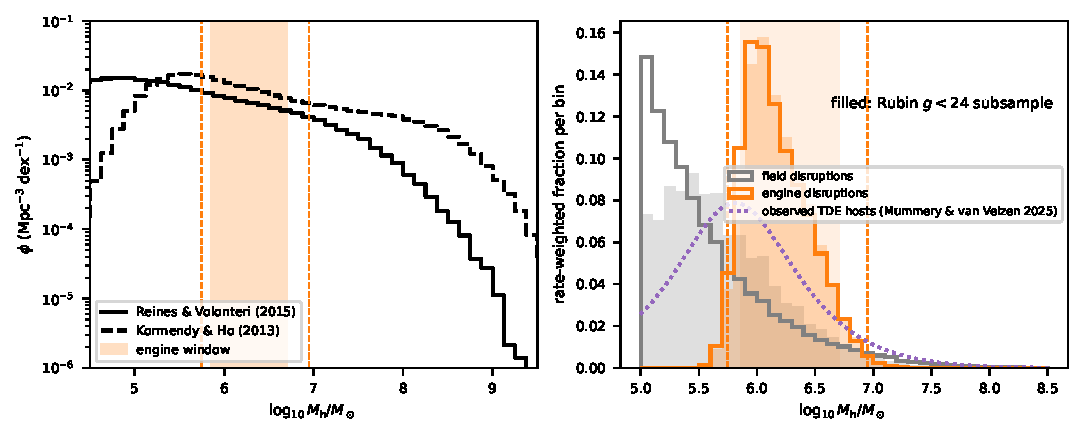
\includegraphics[width=\textwidth]{figures/bhmf.pdf}
\caption{Left: local black hole mass function implied by the galaxy stellar mass function and the two adopted $M_{\rm h}$--$M_{\ast}$ relations. The shaded band marks the engine window between the fiducial $M_{\rm floor}$ and $M_{\rm ceil}$, and the dashed lines the outer $1\sigma$ soft edges, $0.12$~dex below the floor and $0.25$~dex above the ceiling, of the log-normal scatter from which each nucleus's own floor and ceiling are drawn. Right: rate-weighted black hole mass distributions of the field (gray) and engine (orange) disruptions in the fiducial model, with the same window and edges. Filled histograms show the subsets brighter than $g = 24$ at peak, the \lsst-detectable population. The dotted purple curve is the black hole mass distribution that \citet{Mummery:2025a} fit to the observed TDE population from its late-time UV plateau luminosities (their Equation~1, with $\log M_{c} = 5.8$ and $\alpha_{h} = -0.85$; the low-mass slope is unconstrained and drawn here as $\alpha_{l} = 1$), read as a density per logarithmic mass, without their Hills-mass suppression, and normalized to the area of the detected field histogram; it describes a flux-limited optical sample and so compares with the filled histograms. The engine distribution is dominated by nuclei that have just crossed their floor through accretion and are still close to it, with a tail of engines seeded inside the window that have grown toward the ceiling.}
\label{fig:bhmf}
\end{figure*}

We draw host galaxies from the local galaxy stellar mass function, using the double-Schechter fit of \citet{Baldry:2012a} for $M_{\ast} \geq 10^{8}~\msun$, and assign black hole masses through the $M_{\rm h}$--$M_{\ast}$ relation. Because the engine is a low-mass phenomenon, the choice of relation at $M_{\ast} \lesssim 10^{10}~\msun$ matters. We adopt the relation of \citet{Reines:2015a} for local AGN, which lies roughly an order of magnitude below the ellipticals-only relation of \citet{Kormendy:2013a} at fixed stellar mass, with its $0.55$~dex intrinsic scatter, and use the \citet{Kormendy:2013a} relation as an alternative. The resulting black hole mass functions are shown in Figure~\ref{fig:bhmf}, with the engine window marked. The window's edges are drawn sharp there and treated as sharp throughout, but in nature the transition into and out of the engine state is smooth, and it is worth estimating over what range. The floor scales as $M_{\rm floor} \propto f_{\ast}^{1.64}$ \citep{Guillochon:2026a}, so the allowed flattening range $0.18 \le f_{\ast} \le 0.25$ alone spreads it over $5$--$9 \times 10^{5}~\msun$, about $\pm 0.12$~dex around the midpoint value; the ratio of tidal to ambient momentum that sets the ceiling falls as $\simeq M_{\rm h}^{-1.4}$ from $9.4$ at $10^{6}~\msun$ to unity at $5 \times 10^{6}~\msun$, so a factor of two in the rate normalization or in the Bondi efficiency $f_{\rm B}$ moves $M_{\rm ceil}$ by a factor of $1.6$, about $\pm 0.2$~dex. Nucleus-to-nucleus variation in $f_{\ast}$, $f_{\rm B}$, and the collision normalization should therefore blur the lower edge by $\sim 0.1$~dex and the upper edge by $\sim 0.2$--$0.3$~dex. We apply these as the widths of the window in the Monte Carlo: each nucleus draws its own floor and ceiling from log-normal distributions of width $0.12$ and $0.25$~dex about the values of Table~\ref{tab:engine}, and the dashed lines in Figure~\ref{fig:bhmf} mark the outer $1\sigma$ soft edges on either side of the shaded hard window. The location and width of the band are unaffected; what the soft edges remove is the pile-up of freshly switched-on engines at a single mass. Below $10^{6}~\msun$ the occupation fraction is uncertain \citep{Miller:2015a,Greene:2020a}; since $M_{\rm floor}$ sits at the edge of this regime, we bracket the results with occupation fractions of unity and of a fit to the \citet{Miller:2015a} constraint that declines to $0.2$ at $M_{\ast} = 10^{8}~\msun$.

Two further quantities are needed for each host. The first is the number density of galaxies in a post-starburst phase, $n_{\rm PSB} \simeq 2 \times 10^{-5}~{\rm Mpc}^{-3}$ \citep{French:2018a,Pattarakijwanich:2016a}, which we distribute in stellar mass as the mass function weighted by a lognormal preference for $M_{\ast} \sim 10^{10.2}~\msun$. The second is the redshift distribution, which enters only through survey volumes and $K$-corrections; we place hosts uniformly in comoving volume to $z = 1$ and neglect evolution in either mass function over that range.

\subsection{Which nuclei host engines}\label{subsec:occupation}

The quantity that most directly controls the size of the engine population is $f_{\rm eng}(M_{\rm h}, t)$, the fraction of post-starburst nuclei of black hole mass $M_{\rm h}$ that host an active engine at time $t$ after the burst. \citet{Guillochon:2026a} supplies a model for it. A nucleus whose black hole is seeded within the window at the time of the burst runs immediately, and runs until its disk is exhausted at $t_{\rm gas}$ or its cusp is consumed at $t_{\rm cusp}$, whichever comes first; a nucleus seeded below $M_{\rm floor}$ is silent until ambient accretion at $f_{\rm Edd} \simeq 0.05\, f_{\rm B,-3}$ carries it across, after
\begin{equation}
t_{\rm on} \simeq 8.8 \times 10^{8}
\left(\frac{f_{\rm Edd}}{0.05}\right)^{-1}
\left(\frac{\epsilon}{0.05}\right)
\frac{\ln\left(M_{\rm floor}/M_{\rm i}\right)}{1.99}~{\rm yr}.
\label{eq:ton}
\end{equation}
We implement this as a Monte Carlo over $4 \times 10^{5}$ post-starburst hosts. For each we draw a stellar mass, a seed black hole mass from the relation of Section~\ref{subsec:hosts}, a burst age uniform in $\log t$ between $10^{8}$ and $2 \times 10^{9}$~yr \citep{French:2018a}, and the nucleus's own $M_{\rm floor}$ and $M_{\rm ceil}$ from the soft edges of Section~\ref{subsec:hosts}; we evolve the black hole through Equation~(\ref{eq:ton}) and mark it as an engine if $t_{\rm on} < t < t_{\rm on} + \tau$. In our fiducial model the disk is resupplied from the $\sim 10^{9}~\msun$ circumnuclear reservoirs of post-starburst galaxies, three orders of magnitude above the disk mass the equilibrium requires, so the lifetime is the cusp consumption time, $\tau = t_{\rm cusp}$; a ``gas-limited'' variant takes $\tau = t_{\rm gas}$ evaluated at the switch-on mass, which is the lifetime of an isolated disk. The black hole continues to grow at $f_{\rm Edd}$ during the engine phase, with an $e$-folding time of $4.4 \times 10^{8}$~yr, and we evaluate $\gameq$ at its current mass; engines that grow past $M_{\rm ceil}$ switch off.

The black holes in these nuclei are not static, and the choice of when the $M_{\rm h}$--$M_\ast$ relation applies matters. The relation of \citet{Reines:2015a} is measured for local AGN, that is, for black holes that are accreting, which is the appropriate comparison sample for nuclei that the engine model requires to be fed at $f_{\rm Edd} \simeq 0.05$; but a black hole accreting at that rate grows by a factor of $e$ every $4.4 \times 10^{8}$~yr, or by an order of magnitude over the $\sim 10^{9}$~yr post-starburst phase, if gas is present throughout. In our fiducial model the relation describes the black holes as they are observed today, at the end of the accretion episode, so the seed at the burst is smaller by $\exp(-t/4.4 \times 10^{8}~{\rm yr})$ and nuclei that would have been inside the window at the burst are instead below the floor and switch on later; this is the reading under which the black holes in the relation are the same actively growing objects the engine describes. In a ``burst-epoch'' variant the relation instead gives the mass at the time of the burst and growth begins only when the engine switches on, which is appropriate if the ambient inflow is itself a product of the engine. The two bracket the ignorance about whether the post-starburst inflow feeds the black hole before the engine exists, and Section~\ref{subsec:variants} shows that the difference is one of the largest in the calculation. There is now direct evidence that the relevant hosts do carry small black holes: \citet{Ramsden:2026a} find that the quenched TDE hosts of $M_{\rm gal} = 10^{9.6}$--$10^{10.5}~\msun$ harbor black holes systematically less massive ($M_{\rm h} \lesssim 10^{6.5}~\msun$) than star-forming galaxies of the same stellar mass, reversing the usual trend, and argue that these galaxies were quenched by a process that also hindered black hole growth. Post-starburst hosts of $10^{10}~\msun$ carrying black holes at or below the \citet{Reines:2015a} value of $10^{6.4}~\msun$, in the engine window, is what both of our variants assume; the fiducial one additionally places them near the floor at the burst. We do not model the rapid growth during the merger-driven starburst itself, which precedes the phase we consider and is what the local relation, whichever epoch it describes, has already absorbed.

A parameter that this model does not supply is the fraction $\fspark$ of post-starburst nuclei that were ever sparked. \citet{Guillochon:2026a} suggested black hole mergers as the sparking mechanism but did not estimate their efficiency. We treat $\fspark$ as a free parameter that multiplies the engine rate density together with $\lamc$; only the product $\fspark \lamc$ is constrained by the rate budget of Section~\ref{subsec:budget}.

\subsection{Disruption rates and the disrupted stars}\label{subsec:rates}

Every nucleus, engine or not, disrupts stars at the rate set by two-body relaxation. For the field population we adopt the loss-cone rate of \citet{Stone:2016a},
\begin{equation}
\Gamma_{\rm field} \simeq 2.9 \times 10^{-5} \left(\frac{M_{\rm h}}{10^{8}~\msun}\right)^{-0.404}~{\rm yr}^{-1},
\label{eq:gfield}
\end{equation}
a fit to the rates implied by the observed nuclear surface brightness profiles of nearby galaxies, and restrict the field to $M_{\rm h} \geq 10^{5}~\msun$, the range over which that fit is calibrated. For engines we use Equation~(\ref{eq:gameq}). Across the engine window the enhancement over the field rate is a factor of $30$--$100$.

The stellar mass function of disrupted stars follows \citet{Kochanek:2016a}: a \citet{Kroupa:2001a} initial mass function truncated at the main-sequence turnoff of a population of the host's age and weighted by the disruption cross-section, which in the full-loss-cone regime scales as the tidal radius $r_{\rm t} \propto R_{\ast} M_{\ast}^{-1/3}$. For post-starburst hosts with burst ages of $10^{8}$--$10^{9}$~yr, the burst population contains stars up to $2.5$--$6~\msun$, which are disrupted preferentially both because of their larger radii and because of their shorter lifetimes relative to the age spread \citep[the regime treated by][]{Mockler:2022a}. The engine cusp contains both the pre-existing old population and the stars formed in the burst, and we do not know their ratio; we draw half of the engine disruptions from each in the fiducial model and show the two limiting cases as variants. Field disruptions are drawn from a $10$~Gyr population.

The impact parameter $\beta \equiv r_{\rm t}/r_{\rm p}$ is drawn from the distribution appropriate to the loss-cone regime. \citet{Guillochon:2026a} found the engine cusp to sit near $q_{\ast} \sim 1$, with the loss cone full at the sphere of influence ($q_{\ast} = 12\, \mhsix^{-0.33}$ at $f_{\ast} = 0.22$) and diffusive inside a critical radius $r_{\rm crit} \simeq 0.3\, a_{\rm h}$. Stars entering from the full-loss-cone region arrive with ${\rm d}N/{\rm d}\beta \propto \beta^{-2}$ between the minimum-disruption $\beta$ and the capture limit $r_{\rm p} = 4\, r_{\rm g}$ \citep{Hills:1975a,Kesden:2012a}; those from the diffusive region random-walk across the loss-cone boundary and graze the star at $\beta$ just above the partial-disruption threshold \citep{Stone:2016a}. We assign $70\%$ of engine disruptions to the full-loss-cone regime and the remainder to the diffusive one. For the field we follow \citet{Stone:2016a}, whose pinhole fraction falls from $\simeq 0.6$ at $10^{6}~\msun$ to $\lesssim 0.1$ at $10^{8}~\msun$. The mass-dependent threshold for disruption is handled through the scaled impact parameter of \mosfit (Section~\ref{subsec:partial}). We exclude stars whose tidal radius lies inside the capture radius, which removes solar-type stars above $M_{\rm h} \simeq 10^{8}~\msun$ but has no effect on the engine window.

\subsection{A first rate budget}\label{subsec:budget}

The comoving number density of post-starburst galaxies is $n_{\rm PSB} \sim 2 \times 10^{-5}~{\rm Mpc}^{-3}$. If every one hosted an active engine at $\gameq \simeq 10^{-2}$~yr$^{-1}$, the engine contribution to the volumetric TDE rate would be $\sim 2 \times 10^{-7}~{\rm Mpc}^{-3}~{\rm yr}^{-1}$, comparable to the {\it entire} observed optical rate of $\dot{n}_{\rm obs} \simeq 3 \times 10^{-7}~{\rm Mpc}^{-3}~{\rm yr}^{-1}$ \citep{vanVelzen:2018a,Yao:2023a}. The Monte Carlo of Section~\ref{subsec:occupation} shows how far below this the engine population falls, and why. Most post-starburst nuclei spend most of the phase either waiting to cross $M_{\rm floor}$ or having exhausted their cusp: in the fiducial model the time-averaged active fraction is $0.21$, the mean rate per post-starburst galaxy is $1.8 \times 10^{-3}$~yr$^{-1}$, and the engine rate density for $\fspark \lamc = 1$ is
\begin{equation}
\dot{n}_{\rm eng} \simeq 3.6 \times 10^{-8}~{\rm Mpc}^{-3}~{\rm yr}^{-1}.
\label{eq:budget}
\end{equation}
The lifetime matters as much as the rate. If the disk is not resupplied, the gas-limited lifetime of Equation~(\ref{eq:tgas}) is only $2.7 \times 10^{7}$~yr at $M_{\rm floor}$, against a post-starburst phase of $\sim 10^{9}$~yr, and the active fraction falls to $0.08$ and $\dot{n}_{\rm eng}$ to $1.0 \times 10^{-8}~{\rm Mpc}^{-3}~{\rm yr}^{-1}$ (Section~\ref{subsec:variants}). Post-starburst hosts account for roughly a third of the optically selected sample \citep{French:2016a,Hammerstein:2021a}, or $\dot{n}_{\rm PSB} \simeq 10^{-7}~{\rm Mpc}^{-3}~{\rm yr}^{-1}$, and $1 - \fom \simeq 78\%$ of engine disruptions are unobscured (Section~\ref{subsec:screen}). For engines to supply the post-starburst TDEs therefore requires
\begin{equation}
\fspark\, \lamc \simeq 2.8,
\label{eq:fspark}
\end{equation}
rising to $\simeq 10$ for an isolated disk. Since $\fspark \leq 1$, the engine hypothesis supplies the post-starburst rate only if the collision normalization sits a factor of a few above its fiducial value, well within its two-decade uncertainty, and only if the circumnuclear disk is fed from outside; an isolated disk falls short by an order of magnitude. We regard this as a useful outcome: the population synthesis is a test with an identifiable failure mode, not a fit with free normalization. In what follows we quote engine yields per unit $\fspark \lamc$ and also for the value that reproduces $\dot{n}_{\rm PSB}$, which we call the rate-matched normalization.

\section{The Light Curve Model}\label{sec:lightcurves}

\subsection{\mosfit}\label{subsec:mosfit}

We generate light curves with the TDE module of \mosfit \citep{Guillochon:2018a,Mockler:2019a}, using version 2.0 of the code. Relative to the released 1.x versions, \mosfit 2.0 changes none of the physics but makes a population calculation of this size practical. The viscous delay, previously evaluated by a 1000-point logarithmic quadrature of the convolution $L(t) = T_{\rm visc}^{-1}\int_{0}^{t} \epsilon \dot{M}(t')\, c^{2} e^{(t'-t)/T_{\rm visc}}\, {\rm d}t'$ at every output time, is now computed as the exact integral of the same piecewise-linear interpolant of the fallback rate through a compiled exponential recurrence, which agrees with the old quadrature to a relative precision of $10^{-4}$ (the residual is the quadrature's own convergence error) and is $\sim 500$ times faster; spectral energy distributions are carried as rectangular arrays and integrated against filter curves interpolated once onto the model wavelength grid, with the blackbody, extinction, and photometry modules vectorized over unique bands; and the fallback engine caches the stellar-structure coefficients and interpolates the hydrodynamic library with array operations that reproduce the previous engine's output exactly. Together these make a full multi-band light curve cost $\sim 10$~ms, so that the $\sim 2 \times 10^{5}$ light curves behind this paper are computed in under an hour on a laptop. The model maps a black hole mass, stellar mass, and scaled impact parameter onto a fallback rate through the hydrodynamical library of \citet{Guillochon:2013a}, with the stellar radius from the \citet{Tout:1996a} mass--radius relation; converts fallback into luminosity with an efficiency $\epsilon$ and a viscous delay $T_{\rm visc}$; applies a soft Eddington cap; and emits the result from a photosphere whose radius scales with luminosity as $R_{\rm ph} = R_{\rm ph,0}\, a_{\rm p} (L/L_{\rm Edd})^{l}$, bounded below by the circularization radius and above by the semi-major axis of the most bound debris. The output is a blackbody spectral energy distribution at each time, from which \mosfit computes photometry in any filter in the SVO Filter Profile Service. We use the model in its forward direction only, evaluating it at the parameters of each synthetic event rather than fitting, at a cost of $\sim 0.05$~s per event. Filters not previously registered with \mosfit, the \euclid VIS and NISP bands, are added through the code's filter-rule mechanism, and the six \spherex detector arrays are represented by top-hat bands spanning each array's wavelength range.

Fits of this model to the optically selected TDE sample \citep{Mockler:2019a,Nicholl:2022a,Hammerstein:2023a} provide empirical distributions for the parameters the physics does not fix, $\epsilon$, $T_{\rm visc}$, $R_{\rm ph,0}$, and $l$; the viscous time is treated separately in Section~\ref{subsec:darkyear}. We draw them jointly from the posterior medians of the 21 events fit by \citet{Nicholl:2022a}, with $0.1$~dex of jitter, which preserves the correlation between $R_{\rm ph,0}$ and $l$ that those fits exhibit, and treat them as independent of the host environment. This is the central assumption of the light curve model: that a disruption in an engine nucleus produces the same intrinsic flare as a disruption of the same star by the same black hole in the field, and differs only in what happens to that light afterward. \citet{Nicholl:2022a} also report a nearly linear correlation between $\epsilon$ and $M_{\rm h}$; because the engine population sits at the low-mass end of the fitted sample, we run a variant in which $\epsilon$ is rescaled as $M_{\rm h}^{0.97}$ from each event's fitted mass to the synthetic one. We discuss the ways in which the environment-independence assumption may fail in Section~\ref{subsec:caveats}.

\subsection{Circularization and the dark year}\label{subsec:darkyear}

The viscous-delay parameter deserves separate comment, because the empirical distribution we draw it from is the one quantity in Table~\ref{tab:params} that is known to be biased by selection. \citet{Guillochon:2015a} followed the debris stream through many windings around a spinning black hole and showed that relativistic precession deflects the thin stream out of its own path, so that the self-intersection that begins circularization occurs only after several orbits of the most bound material (a ``dark year''), and that the intersection radius, which sets the circularization time, is controlled by the apsidal precession per orbit and hence by $r_{\rm p}/r_{\rm g} \propto \beta^{-1} M_{\rm h}^{-2/3}$. Around massive black holes the streams collide violently near pericenter and the flare follows the fallback rate after a fixed delay; around black holes of $M_{\rm h} \lesssim 10^{6}~\msun$ the intersection occurs far out, the viscous time exceeds the fallback time by an order of magnitude or more, and the flare is slowed: longer, fainter, sub-Eddington, and with its late-time decline converging toward $t^{-1}$ rather than tracing the fallback rate. The transition from mostly slowed to mostly prompt flares occurs near $10^{7}~\msun$ for a thick-disk viscosity, and prompt flares around $10^{6}~\msun$ black holes require $\beta \gtrsim 5$. Because slowed flares are harder to find, \citet{Guillochon:2015a} argued that optical samples are biased toward the prompt minority, and the fits of \citet{Mockler:2019a} and \citet{Nicholl:2022a}, which find viscous times of no more than a few days for every event, are consistent with that bias rather than evidence against long delays.

This matters for the engine population more than for most, because the engine window sits entirely in the mass range where slowed flares should dominate. Our fiducial model therefore sets the viscous time from the encounter rather than drawing it from the fitted sample, and a ``prompt'' variant uses the fitted values instead: $\log_{10}(T_{\rm visc}/t_{\rm peak}) = \mu + 0.5\,\xi$, with $\xi$ a unit normal deviate, $\mu = 1.0 + 2.1 \log_{10}[(r_{\rm p}/r_{\rm g})/47]$ clipped to $[-1.5, 2]$, and $t_{\rm peak}$ the fallback peak time of \citet{Guillochon:2013a}. This reproduces the three anchors of \citet{Guillochon:2015a}: a slowdown of an order of magnitude for a solar-type star at $\beta = 1$ around $10^{6}~\msun$ ($r_{\rm p}/r_{\rm g} = 47$), prompt flares at $\beta \gtrsim 5$ around such black holes, a transition to mostly prompt flares near $10^{7}~\msun$, and a cap of $\sim 100\, t_{\rm peak}$ set by the time for the stream to fill $4\pi$. \mosfit implements the delay as an exponential smoothing of the fallback rate on the timescale $T_{\rm visc}$ \citep{Mockler:2019a}, so the prescription changes the shape of every light curve in the window, and we apply it to the field population as well; the dark period that precedes circularization, by contrast, shifts the flare in time without changing its shape and we do not track it, except to note that it delays the echo of Section~\ref{subsec:echo} by the same amount. The prescription is a parameterization of a Monte Carlo that itself depends on the assumed disk viscosity, and we treat it as a bracket rather than a prediction.

\subsection{Partial disruptions}\label{subsec:partial}

The fallback library underlying \mosfit spans the full range of encounters from the onset of mass loss to deep plunges, for $\gamma = 5/3$ and $\gamma = 4/3$ polytropes. \mosfit parameterizes the encounter by a scaled impact parameter $b$ such that $b = 0$ is the minimum disruption and $b = 1$ the shallowest full disruption for either polytrope, with $\beta = 0.5 + 0.4\,b$ for $\gamma = 5/3$ and $\beta = 0.6 + 1.25\,b$ for $\gamma = 4/3$ below $b = 1$, and interpolates between the polytropes for stars of $0.3$--$1~\msun$. We draw physical $\beta$ as described in Section~\ref{subsec:rates} and invert this map for each star. Because a $\gamma = 4/3$ star needs $\beta \geq 1.85$ to be fully disrupted while a $\gamma = 5/3$ star needs only $\beta \geq 0.9$, the same $\beta^{-2}$ distribution yields a full-disruption fraction of $\simeq 0.54$ for low-mass stars but only $\simeq 0.3$ for stars above a solar mass. The young engine population is therefore more partial than the old one at fixed loss-cone regime, and this is one of the channels through which the engine shapes the light curves.

The library reproduces the two features of partial disruptions that matter observationally. The bound mass falls steeply with decreasing $\beta$ below the full-disruption threshold, from $\Delta M \simeq 0.4$--$0.5~M_{\ast}$ for a full disruption to $\sim 1\%$ of the star at $b = 0.2$, so that grazing encounters are faint. The late-time decline is steeper than $t^{-5/3}$: we measure ${\rm d}\ln L/{\rm d}\ln t \simeq -2.0$ between $200$ and $600$~d for $b \lesssim 0.5$ against $-0.7$ to $-0.9$ for $b \geq 1$, consistent with the $t^{-9/4}$ asymptote of \citet{Coughlin:2019a} and with the simulations of \citet{Miles:2020a} and \citet{Nixon:2021a}, although the shallower full-disruption slopes at these times reflect the Eddington cap and the photosphere prescription rather than the fallback rate alone. We do not attempt to model the repeated flares that a surviving core on a bound orbit can produce \citep{Payne:2021a,Wevers:2023a,Lin:2024a,Somalwar:2025a,Hinkle:2024a,Liu:2025a}: in the engine the stars arrive on nearly parabolic orbits from the sphere of influence with periods of $10^{3}$--$10^{4}$~yr, so any return is not observable, though the compressed cusp does raise the chance that two unrelated disruptions overlap (Section~\ref{subsec:agn}).

\citet{Angus:2026a} caution that the polytropic fallback grid is a limitation when parameters are {\it inferred} from partial disruptions: fits to known repeating partial TDEs converge on full-disruption solutions with unphysically low stellar masses, because a lower $M_{\ast}$ at higher $b$ produces a light curve similar to that of a more massive star stripped partially. In the forward direction this degeneracy does not bias the synthetic population, since we specify $M_{\ast}$ and $b$ rather than recover them, but it does mean that the light curves of the young, partially disrupted engine population will be interpreted by a fitter as those of fully disrupted low-mass stars. We return to what this implies for testing the engine in Section~\ref{subsec:recovery}. The grid's more fundamental limitation, that main-sequence stars of a few solar masses are not $\gamma = 4/3$ polytropes and that realistic structure changes both the threshold $\beta$ and the shape of the fallback curve \citep{Golightly:2019a,Law-Smith:2020a,Ryu:2020c}, applies equally in both directions; the STARS library of \citet{Law-Smith:2020a} would be the natural replacement once its partial-disruption coverage matches that of the polytropic grid.

\subsection{Parameter distributions}\label{subsec:params}

Table~\ref{tab:params} (Appendix~\ref{app:tables}) lists the distributions from which each event is drawn: black hole masses from the mass function weighted by the disruption rate, stellar masses from the present-day mass function weighted by the tidal cross-section, impact parameters from the loss-cone regime, photosphere and efficiency parameters from the 21 fitted events, viscous times from the encounter geometry, host extinction from the fitted columns, and isotropic disk orientations and comoving-volume redshifts to $z = 1$. The black hole mass distribution of engine disruptions is the mass function weighted by $f_{\rm eng}(M_{\rm h})\, \gameq(M_{\rm h})$. Because $f_{\rm eng}$ vanishes below $M_{\rm floor}$, $\gameq \propto M_{\rm h}^{-0.84}$, and in the fiducial model most nuclei enter the window from below by accretion, the distribution is peaked just above $7 \times 10^{5}~\msun$ (Figure~\ref{fig:bhmf}): the 16th, 50th, and 84th percentiles are $10^{5.90}$, $10^{6.12}$, and $10^{6.47}~\msun$, the tail being engines seeded inside the window that have grown toward the ceiling, and the peak broadened by the soft floor of Section~\ref{subsec:hosts}. This is far below the median of the optically selected sample near $10^{6.5}$--$10^{6.7}~\msun$ \citep{Mockler:2019a,Yao:2023a,Nicholl:2022a}. The concentration at the floor is not generic: if the lifetime is gas-limited it rises as $\mhsix^{2.33}$ faster than the rate falls, and the distribution moves to a median of $10^{6.4}~\msun$ (Section~\ref{subsec:variants}). Engine disruptions are super-Eddington in fallback at peak by factors of $10$--$100$, and were circularization prompt the radiated luminosity would be pinned near $L_{\rm Edd}$; with the slowed circularization of Section~\ref{subsec:darkyear} the accretion rate is spread over the viscous time and most flares fall below the cap. This is the regime in which radiatively driven outflows are expected \citep{Metzger:2016a,Dai:2018a}, and in which the cooling-envelope description of \citet{Metzger:2022a} and \citet{Sarin:2024a} may be more appropriate than a fallback-following one \citep{Mummery:2025b}; we note where this matters.

Each engine is assigned a disk normal drawn isotropically, and the inclination $i$ of the observer's sightline to that normal determines both the extinction (Section~\ref{subsec:screen}) and the echo transfer function (Section~\ref{subsec:echo}). Host extinction for both populations is drawn from the fitted column densities of \citet{Nicholl:2022a}, and field disruptions receive no circumnuclear reprocessing beyond the small covering factors inferred by \citet{Jiang:2021b}.

\subsection{The circumnuclear disk as a screen}\label{subsec:screen}

The disk occupies $|\cos i| < \fom$, where $i$ is measured from the disk normal, so a fraction $\fom$ of randomly oriented sightlines pass through it. Along those sightlines the extinction has two components. The inter-cloud medium contributes the $\Av \simeq 50$ of Table~\ref{tab:engine}, corresponding to $N_{\rm H} \simeq 10^{23}~{\rm cm}^{-2}$ at the Galactic gas-to-dust ratio \citep{Bohlin:1978a}. The clouds themselves are much thicker: a sightline through a single cloud intercepts $N_{\rm H} \simeq 2 n_{\rm MC} R_{\rm MC} \simeq 8 \times 10^{23}~{\rm cm}^{-2}$, or $\Av \sim 400$. Because the first equilibrium condition requires the clouds to cover the disk as seen from the black hole, most disk sightlines will intercept at least one. We therefore treat $\Av = 50$ and $\Av = 400$ as limiting cases, and note that the difference is immaterial in the optical and ultraviolet, where either value is completely opaque, but decisive in the near- and mid-infrared. We use the extinction curve of \citet{Cardelli:1989a} with $R_{V} = 5$, appropriate to dense gas, out to $3~\um$, and the mid-infrared law of \citet{Indebetouw:2005a} beyond, scaled to the $K$-band value of the same curve. The resulting dimming in each band is listed in Table~\ref{tab:screen}: an engine disruption seen through the inter-cloud medium is dimmed by $3.7$~mag in \wise W1 and $2.9$~mag in W2, and would remain detectable in the mid-infrared at $z \lesssim 0.03$, while one seen through a cloud is dimmed by $30$ and $23$~mag and is detectable only through its dust emission. The near-infrared bands of \euclid and \romantel sit in between: $A_V = 50$ costs $10$~mag in $H_{\rm E}$ and $7$~mag in F213, enough to hide any engine flare beyond the nearest hosts.

The remaining $1 - \fom \simeq 78\%$ of sightlines view the nucleus over the disk. We assume these are unobscured apart from host-galaxy extinction, but we flag this as an assumption. Post-starburst nuclei drive molecular outflows \citep{Alatalo:2015a}, the engine's own Bondi inflow must arrive from somewhere, and any material above the disk plane with $N_{\rm H} \gtrsim 10^{21}~{\rm cm}^{-2}$ would add appreciable optical extinction. We treat a polar extinction $A_{V,{\rm pole}}$ as a nuisance parameter with a fiducial value of zero.

The immediate consequence is that the obscured fraction of engine disruptions is $\fom$, and that the dependence is on inclination alone: an engine is either seen or not, with no intermediate regime in the optical. This is a sharper statement than that of most obscured-TDE models and is testable with a sample of infrared-selected events in post-starburst hosts.

\begin{deluxetable}{lcccc}
\tablecaption{Dimming by the disk in selected bands \label{tab:screen}}
\tablehead{\colhead{Band} & \colhead{$\lambda_{\rm eff}$ ($\um$)} & \colhead{$A_\lambda/\Av$} & \colhead{$\Av = 50$} & \colhead{$\Av = 400$}}
\startdata
UVW2 & 0.21 & 1.898 & 94.9 & 759 \\
$g$ & 0.47 & 1.131 & 56.6 & 452 \\
$z$ & 0.87 & 0.589 & 29.4 & 235 \\
\euclid $Y_{\rm E}$ & 1.07 & 0.421 & 21.0 & 168 \\
\euclid $H_{\rm E}$ & 1.74 & 0.192 & 9.6 & 77 \\
\romantel F213 & 2.11 & 0.141 & 7.0 & 56 \\
\spherex 2.4--3.8~$\um$ & 3.12 & 0.075 & 3.8 & 30 \\
W1 & 3.35 & 0.074 & 3.7 & 30 \\
W2 & 4.60 & 0.057 & 2.9 & 23 \\

\enddata
\tablecomments{Extinction curve of \citet{Cardelli:1989a} with $R_V = 5$ to $3~\um$, \citet{Indebetouw:2005a} beyond. Dimming in magnitudes. Generated by {\tt scripts/postprocess.py}.}
\end{deluxetable}

\subsection{The disk as a dust reprocessor}\label{subsec:echo}

The disk absorbs a fraction $\fom$ of the flare's radiation and re-emits it in the infrared. Dust echoes of nuclear transients are usually modeled as spherical shells \citep{Lu:2016a,vanVelzen:2016a}, but the geometry matters: \citet{Eyles-Ferris:2026a} shows that a ring rather than a shell reproduces the observed preference of X-ray-bright TDEs for infrared counterparts, produces brighter and later-rising echoes on-axis and double-peaked ones off-axis, and lets the observing angle be inferred from the echo alone; \citet{Tuna:2025a} find with time-dependent radiation transport that polar observers of a dusty torus see faster, brighter, shorter echoes than equatorial ones; and \citet{Wu:2026a} show that a precessing disk imprints variability on the echo of even a static ring. The engine's disk is a ring by construction, and the inclination dependence these authors derive is what the transfer function below encodes. The covering factor is the other point of contact: \citet{Hinkle:2024b} measure dust covering fractions of $0.05$--$0.9$ (mean $0.3$) from the mid-infrared echoes of ambiguous nuclear transients and interpret them as tori, against $\lesssim 0.01$ for optically selected TDEs \citep{Jiang:2021b}; the engine predicts $\fom = 0.22$, at the AGN-like end of that range, for every post-starburst nucleus that hosts one. Two properties of the engine geometry make the resulting echo unlike those observed to date.

The first is the delay. The inner edge of the disk is at $r_{\rm in} = \rb - R_{\rm MC} \simeq 4.1\, \mhsix^{0.91}$~pc, so an element of the disk at azimuth $\phi$ re-emits with a delay
\begin{equation}
\tau(\phi, i) = \frac{r_{\rm in}}{c}\left(1 - \sin i \cos\phi\right)
\end{equation}
relative to the direct light, where $\phi = 0$ is the near side. For $r_{\rm in} = 4.1$~pc, $r_{\rm in}/c = 13.3$~yr, and because $R_{\rm MC}$ grows faster with mass than $\rb$, $r_{\rm in}$ scales as $\mhsix^{0.91}$ across the window. A face-on engine ($i = 0$) presents a ring at a single delay, and its echo is a delayed copy of the flare, smoothed only by the light-travel spread across the cloud-scale corrugation of the inner face, $R_{\rm MC}/c \simeq 2.3\, \mhsix^{1.49}$~yr. An edge-on engine spreads the same energy over delays from zero to $2 r_{\rm in}/c \simeq 27$~yr. The echo light curve is the convolution of the flare with the transfer function
\begin{equation}
\Psi(\tau; i) = \frac{\fom}{\pi \tau_{0} \sin i}\left[1 - \left(\frac{1 - \tau/\tau_{0}}{\sin i}\right)^{2}\right]^{-1/2},
\quad \tau_{0} \equiv \frac{r_{\rm in}}{c},
\label{eq:transfer}
\end{equation}
for $|1 - \tau/\tau_{0}| < \sin i$ and zero otherwise, which integrates to $\fom$; we normalize it numerically after the cloud-scale smoothing.

The second is the temperature. At $4$~pc from a flare of $L = 10^{44}~{\rm erg~s^{-1}}$, grains reach equilibrium temperatures that depend on their emissivity: $\simeq 440$~K for the $\epsilon_\nu \propto \nu$ graphite grains of \citet{Barvainis:1987a}, whose sublimation radius for such a flare is $\simeq 0.13$~pc, and $\simeq 120$~K for gray grains. The echo therefore peaks at $7$--$25~\um$, in contrast to the $\sim 1000$~K, $\sim 3~\um$ echoes observed from optically selected TDEs \citep{vanVelzen:2016a,Jiang:2016a}. The inner face of the disk is optically thick to the incident ultraviolet, so the echo luminosity $L_{\rm IR}(t) = \int L_{\rm flare}(t')\, \Psi(t - t'; i)\, {\rm d}t'$ is independent of the dust mass, and for a face-on engine peaks at $L_{\rm IR} \simeq \fom L_{\rm peak}$ diluted by the cloud-scale smoothing. We adopt the \citet{Barvainis:1987a} temperature for the fiducial echo photometry and quote the gray-grain value as the alternative.

\subsection{The ambient accretion flow}\label{subsec:agn}

The engine nucleus is not quiescent between disruptions. The Bondi inflow from the inter-cloud gas produces $L_{\rm AGN}/L_{\rm Edd} \simeq 0.05\, f_{\rm B,-3}$, or $L_{\rm AGN} \simeq 6 \times 10^{42}\, f_{\rm B,-3}\, \mhsix~{\rm erg~s^{-1}}$, a low-luminosity AGN, against which the flare must be detected and whose variability, which we do not model, will contribute to the false-positive rate of any infrared echo search. The rate of disruptions is also high enough that flares overlap: at $\gameq = 1.4 \times 10^{-2}$~yr$^{-1}$ the mean interval between events is $\sim 70$~yr, longer than the optical flare duration but comparable to the echo delay, so that an engine viewed face-on will at any moment be displaying the echo of the previous disruption while awaiting the next. Over many cycles the disk maintains a warm dust component at a mean luminosity $\fom \gameq E_{\rm rad} \sim 10^{41}~{\rm erg~s^{-1}}$, which sets a floor to the nuclear mid-infrared emission of any engine.

\section{Results}\label{sec:results}

\subsection{Rates, mass distributions, and the rate budget}\label{subsec:rates_result}

The rate budget of Section~\ref{subsec:budget} is the first result. A fifth of post-starburst nuclei host an active engine at a given moment, and the population is dominated by nuclei that crossed $M_{\rm floor}$ during the post-starburst phase rather than by nuclei seeded inside the window: the switch-on delay of Equation~(\ref{eq:ton}) is $3$--$9 \times 10^{8}$~yr for seeds of $10^{5}$--$4 \times 10^{5}~\msun$, comparable to the burst ages, and a nucleus that crosses the floor at $t_{\rm on}$ has its full cusp lifetime of $1.6 \times 10^{8}$~yr ahead of it. This is why the growing-black hole and resupplied-disk ingredients reinforce one another (Section~\ref{subsec:variants}): the first delivers nuclei to the floor throughout the phase, the second keeps them running once there. The choice of $M_{\rm h}$--$M_\ast$ relation is the most sensitive remaining input: with the \citet{Kormendy:2013a} relation, post-starburst hosts of $10^{10}~\msun$ carry black holes above $M_{\rm ceil}$ even after the growth correction, the active fraction falls to $4\%$, and $\dot{n}_{\rm eng}$ drops by a factor of nine. The occupation-fraction bracket changes $\dot{n}_{\rm eng}$ by only $7\%$, because the engine window sits above the masses where occupation is uncertain, but halves the field rate. The field rate itself, $4.3 \times 10^{-6}~{\rm Mpc}^{-3}~{\rm yr}^{-1}$ for $M_{\rm h} \geq 10^{5}~\msun$, exceeds the observed optical rate by a factor of $14$, the familiar tension between loss-cone theory and optical samples \citep{Stone:2016a,vanVelzen:2018a,Yao:2023a}; it is dominated by black holes of $10^{5}$--$10^{5.5}~\msun$ whose flares are faint and, with slowed circularization, long, and we rescale it to the observed rate when quoting field yields below.

The black hole mass distributions of the two populations (Figure~\ref{fig:bhmf}, right) follow from the window, the lifetime, and the growth history, and not from $\lamc$. The intrinsic field distribution has a median of $10^{5.43}~\msun$ and is flux-limited by \lsst to $10^{5.3}$--$10^{6.3}~\msun$ (median $10^{5.70}$) and by ZTF to $10^{5.7}$--$10^{6.7}~\msun$ (median $10^{6.22}$). The engine distribution is concentrated near the floor, with a median of $10^{6.12}~\msun$; because the brightest engine flares come from the most massive engines, flux limits move the detected subsets upward, to $10^{5.9}$--$10^{6.5}~\msun$ (median $10^{6.16}$) for \lsst and $10^{6.1}$--$10^{6.7}~\msun$ (median $10^{6.38}$) for ZTF. In a shallow survey the engine and field populations are therefore hard to separate by mass alone; in a deep one the engine population sits $0.45$~dex above the field's median and is far narrower, and it is the narrowness, the concentration of post-starburst TDEs into a single decade of mass with a hard lower edge, that is the engine's signature. The observed mass distributions to compare with are the light-curve-derived ones of \citet{Yao:2023a}, which peak near $10^{6.6}~\msun$ for the ZTF sample, the plateau-derived distribution that \citet{Mummery:2025a} fit to reproduce the luminosity functions, and the $89$ optical-flare masses of \citet{Mummery:2026a}; all three describe flux-limited optical samples, so the comparison is with the filled histograms of Figure~\ref{fig:bhmf}, and all three are dominated by the field population unless post-starburst hosts are selected. The \citet{Mummery:2025a} distribution, drawn in Figure~\ref{fig:bhmf}, breaks at $10^{5.8}~\msun$ and falls as $M_{\rm h}^{-0.85}$ above it, so it spans $10^{5.8}$--$10^{7.5}~\msun$ with most of its weight near $10^{6.5}~\msun$: broader and more massive than our \lsst-detected field population, whose median of $10^{5.7}~\msun$ reflects the \citet{Reines:2015a} relation and the $10^{5}~\msun$ floor we impose, and broader than the engine population by a factor of several in width. If the \citet{Mummery:2025a} distribution is the field, the engine would add a narrow component at its low-mass end, just above the break; if the break itself is the engine floor, as its coincidence with $M_{\rm floor}$ invites one to consider, the post-starburst hosts should carry the events in the $10^{5.8}$--$10^{6.5}~\msun$ decade and the star-forming hosts the tail above.

\subsection{Light-curve distributions}\label{subsec:lcdist}

\begin{figure*}[t]
\centering
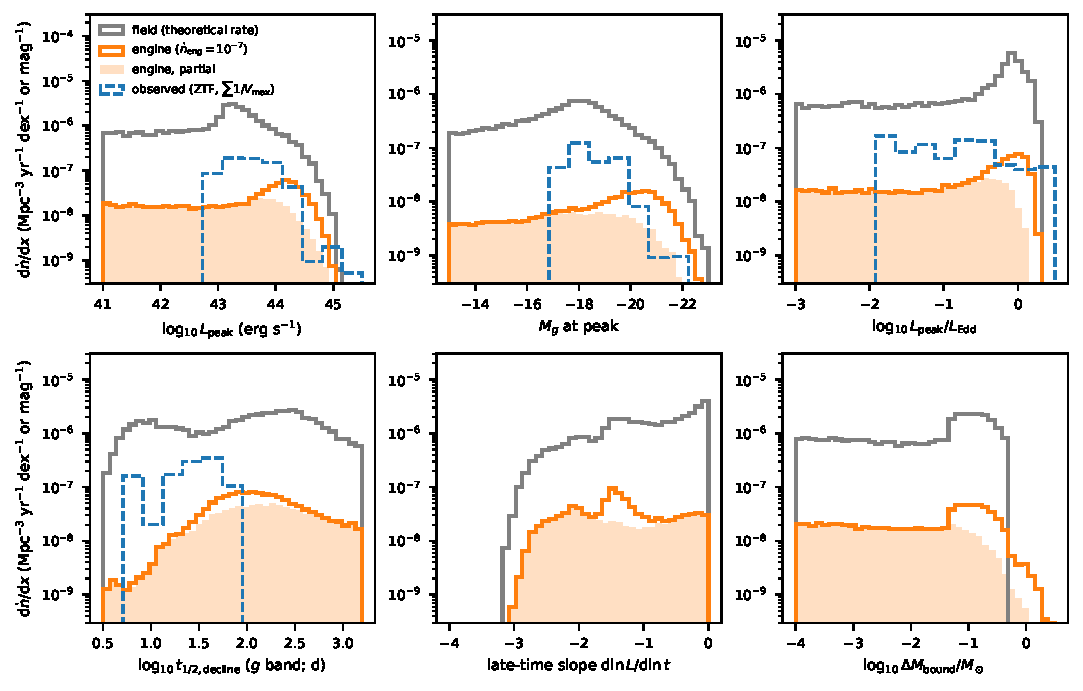
\includegraphics[width=\textwidth]{figures/lcdist.pdf}
\caption{Volumetric rate densities of light-curve properties for the field population at its theoretical rate (gray) and the engine population at the rate-matched normalization $\fspark \lamc = 2.8$ (orange) in the fiducial model; the filled orange histograms isolate the partial disruptions ($b < 1$) among engine events. From left to right and top to bottom: peak bolometric luminosity, peak absolute $g$ magnitude, peak Eddington ratio, rest-frame time for the $g$-band light curve to fade to half its peak, logarithmic slope of the decline between $200$ and $600$~d after peak, and mass bound to the black hole. Dashed blue histograms in the first four panels show the 33 ZTF TDEs of \citet{Yao:2023a}, each contributing its $1/V_{\rm max}$ rate density (with their survey-efficiency correction), so that the observed histograms carry their actual volumetric normalization; they use their blackbody peak luminosity, rest-frame $g$-band peak luminosity, blackbody luminosity over the Eddington luminosity of the host-derived black hole mass, and rest-frame time from peak to half maximum in the $g$ band, in bins three times wider than the models. The half-decline panel uses the same $g$-band definition for the models; the bolometric values are listed in Table~\ref{tab:lcstats}.}
\label{fig:lcdist}
\end{figure*}

Figure~\ref{fig:lcdist} compares the light-curve properties of the two populations, and Table~\ref{tab:lcstats} (Appendix~\ref{app:tables}) lists their percentiles. In summary, the median engine disruption peaks at $10^{43.1}~{\rm erg~s^{-1}}$ and $M_g = -16.5$, $110$~d after first fallback, and declines to half maximum in $270$~d bolometrically ($230$~d in the $g$ band); the median field disruption peaks at $10^{42.6}~{\rm erg~s^{-1}}$ and $M_g = -14.9$ after $150$~d and declines in $560$~d ($440$~d in $g$); and both populations have peak blackbody temperatures near $3.4 \times 10^{4}$~K and radiate $10^{50.4}$--$10^{50.7}$~erg. Three features are set by the engine.

The first is the partial fraction. Partial disruptions make up $71\%$ of engine events and $66\%$ of field events, the difference arising from the engine's full loss cone, which sends stars in with $\beta^{-2}$ down to the minimum-disruption threshold. The stellar age has almost no effect: the partial fraction is $0.72$ for the young half of the engine population and $0.70$ for the old half, because even a $10^{8.5}$~yr population is dominated by stars below $0.5~\msun$ after the $r_{\rm t}$ weighting (median $0.38$ against $0.31~\msun$), and the harder-to-disrupt $\gamma = 4/3$ stars are too rare to move the total. The channel we anticipated in Section~\ref{subsec:partial} is real but subdominant; the loss-cone regime is what matters.

The second is the luminosity of the full disruptions. Engine full disruptions have $L_{\rm peak} = 10^{43.7}$--$10^{44.35}~{\rm erg~s^{-1}}$ (16th--84th percentiles), a narrow range because the engine's mass range is narrow and its black holes sit at the floor, where $L_{\rm Edd} = 10^{44.0}~{\rm erg~s^{-1}}$; a fifth of them are within $10\%$ of the Eddington cap, the rest held below it by the slowed circularization. Their $M_g$ distribution peaks at $-20$, more than a magnitude brighter than the field's full disruptions at $L_{\rm peak} \simeq 10^{43.3}~{\rm erg~s^{-1}}$. The partial disruptions are fainter by $1.7$~dex at the median ($10^{42.3}~{\rm erg~s^{-1}}$) and fill in the luminosity function smoothly from $M_g = -20$ down to $-10$, dominating the population below $M_g = -19$; in the engine they are fainter than in the field by less than the full disruptions are brighter, because the small $\beta$ that makes an encounter partial also makes it slowed.

The third is the timescale, and here the slowed circularization dominates. Engine light curves peak $50$--$210$~d after first fallback ($110$~d median) and decline to half maximum in $100$--$800$~d ($270$~d median), against $150$ and $560$~d for the field, whose smaller black holes are slowed more. Partial disruptions decline more slowly than full ones in both populations ($300$ against $210$~d for engines), the reverse of the prompt case in which the stripped envelope falls back quickly, because the shallow encounters have the largest $r_{\rm p}/r_{\rm g}$ and hence the longest viscous times. The late-time slope between $200$ and $600$~d, ${\rm d}\ln L/{\rm d}\ln t = -1.4^{+0.8}_{-0.7}$ for engines and $-0.9^{+0.6}_{-0.9}$ for the field, is broadened by the same effect: events still within their viscous time at $200$~d have not yet begun to decline as the fallback rate does, so the $t^{-9/4}$ signature of partial disruptions \citep{Coughlin:2019a} survives only in the prompt minority. The engine distributions are narrower than the field's in every timescale because the engine's mass range is.

Figure~\ref{fig:lcdist} also shows the $33$ ZTF TDEs of \citet{Yao:2023a} as summed $1/V_{\rm max}$ rate densities, so that the comparison is between distributions with their actual volumetric normalizations: the field at its theoretical rate, the engine at the rate-matched normalization, and the observed sample at the rate it implies. Where the two can be compared, the luminosities agree. The observed events have $L_{\rm bb} = 10^{43.0}$--$10^{43.8}~{\rm erg~s^{-1}}$ (rate-weighted 16th--84th percentiles; median $10^{43.5}$), $M_g = -17.9$ to $-19.4$, and Eddington ratios of $0.02$--$0.5$ against their host-derived black hole masses; the engine's full disruptions occupy the adjacent decade, $10^{43.7}$--$10^{44.35}~{\rm erg~s^{-1}}$ at Eddington ratios of $0.1$--$1$, and the field's full disruptions are a factor of a few fainter, so that in the panels of peak luminosity and peak magnitude the observed histogram peaks where the field's full disruptions do, half a decade below the engine's, at a height between the two. This agreement has a simple origin and is not a discriminating success: the observed hosts carry black holes of $10^{6.4}~\msun$ at the rate-weighted median ($10^{5.4}$--$10^{7.1}$), the same as the engine events that ZTF would detect in our model ($10^{6.1}$--$10^{6.7}$, median $10^{6.4}$; Table~\ref{tab:yields}) and as the detected field events ($10^{6.2}$), and any population of $10^{6}$--$10^{6.5}~\msun$ black holes radiating within a factor of a few of Eddington lands where the data are. The differences are two. The first is at the faint end: the observed sample contains no event fainter than $L_{\rm bb} = 10^{43}~{\rm erg~s^{-1}}$ or $M_g = -17.6$, whereas both model populations are dominated by partial disruptions a decade fainter. Part of this is selection, since an $M_g = -16$ event passes the ZTF flux limit only within $\sim 60$~Mpc, but the $1/V_{\rm max}$ weighting corrects for exactly that, and the faintest events in the sample, at $M_g \simeq -17.5$ to $-18$, already carry half of the summed rate; the absence of any event a magnitude fainter in a spectroscopically complete sample is therefore a mild but real constraint. It says that partial disruptions are either less common than the $\beta^{-2}$ full loss cone gives, or fainter than the \mosfit fallback scaling makes them, or slowed so much that they fail the ZTF duration and color cuts, which the $300$~d half-decline times of the fiducial model's partial disruptions make plausible. The second difference is the timescale, and it is much larger. \citet{Yao:2023a} measure the half-decline time in the rest-frame $g$ band, and because the \mosfit photosphere shrinks and heats as the luminosity falls, the $g$-band flux drops faster than the bolometric luminosity ($L_g \propto L^{(1+6l)/4}$ on the Rayleigh--Jeans side, or $L^{2.5}$ for $l = 1.5$); the panel of Figure~\ref{fig:lcdist} and the comparison here therefore use the same $g$-band measure for the models, which shortens the engine and field medians from $270$ and $560$~d bolometric to $230$ and $440$~d. The observed values, $15$--$90$~d, remain shorter by a factor of four or more. Both differences are in the direction expected if the optical sample is drawn from the prompt minority: the prompt variant of Section~\ref{subsec:variants} reproduces the observed timescales and luminosities ($M_g = -18.3$ and $-17.5$), while the fiducial populations, in which most flares are slowed, would be found by ZTF only through their brightest, promptest members. The rate-weighted observed distribution is dominated by a handful of nearby events and its shape is correspondingly uncertain, but the offset in timescale does not depend on the weighting; either the slowed majority exists and has largely escaped optical selection, as \citet{Guillochon:2015a} argued, or circularization in this mass range is prompter than the fiducial prescription assumes, and the two possibilities are distinguished by the duration distribution of a deeper, less color-selected sample such as \lsst will provide.

What the engine does not fix is the temperature and the photospheric radius: the peak blackbody temperatures of the two populations, both $3.4 \times 10^{4}$~K at the median, are set by the drawn $R_{\rm ph,0}$ and $l$ and differ only through the Eddington ratio. The variant in which $\epsilon$ scales with $M_{\rm h}$ \citep{Nicholl:2022a} lowers the median engine efficiency by a factor of three ($0.029 \to 0.010$) and the field's by five ($0.029 \to 0.006$). For the engine this moves the full-disruption peak luminosity down by $0.2$~dex, drops the fraction within $10\%$ of the Eddington cap from $19\%$ to $4\%$, fades the median $M_g$ from $-16.5$ to $-15.5$, and lowers the \lsst yield by a fifth; for the field the effect is larger, with the median $M_g$ fading from $-14.9$ to $-12.8$ and the \lsst yield falling by $40\%$. With slowed circularization the engine flares no longer sit at the Eddington cap, so they no longer forget $\epsilon$ as prompt flares of the same black holes would; the engine's relative insensitivity is now only that its black holes are the more massive of the two populations, so its efficiencies are rescaled less.

\subsection{Luminosity functions and obscured fractions}\label{subsec:lf}

\begin{figure*}[t]
\centering
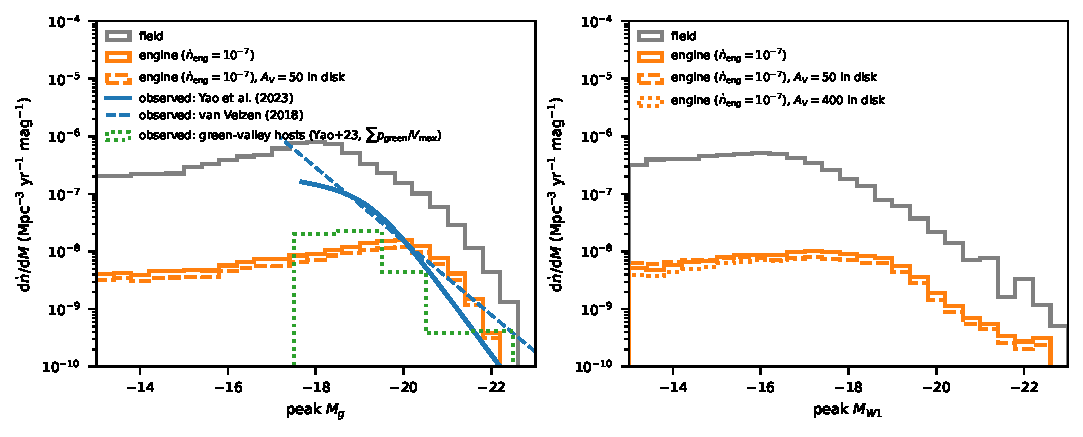
\includegraphics[width=\textwidth]{figures/lf.pdf}
\caption{Peak luminosity functions in the \lsst $g$ band (left) and \wise W1 band (right) for the field population at its theoretical rate (gray) and the engine population at the rate-matched normalization $\fspark \lamc = 2.8$ (orange). Solid lines are intrinsic; dashed and dotted lines include the disk screen with $\Av = 50$ and $400$ for the $\fom$ of sightlines that pass through it. Blue curves show the observed rest-frame $g$-band luminosity functions of optically selected TDEs: the double power law of \citet{Yao:2023a} (solid) and the single power law of \citet{vanVelzen:2018a} (dashed), each over the luminosity range of its sample and converted to a rate density per magnitude. The field rate exceeds the observed optical rate by a factor of $14$; at the observed rate the field curve would lie $1.1$~dex lower.}
\label{fig:lf}
\end{figure*}

Figure~\ref{fig:lf} shows the peak luminosity functions in $g$ and W1, with the engine population at the rate-matched normalization $\fspark \lamc = 2.8$, together with the observed rest-frame $g$-band luminosity functions of \citet{Yao:2023a}, a double power law breaking at $L_g = 1.4 \times 10^{43}~{\rm erg~s^{-1}}$ with slopes of $0.26$ below and $2.58$ above, and of \citet{vanVelzen:2018a}, ${\rm d}\dot N/{\rm d}\log L_g \propto L_g^{-1.6}$. The field luminosity function is flat from $M_g = -14$ to $-19$ and falls steeply brightward of $-19.5$, where the observed one breaks, because its black holes are small and, with slowed circularization, their flares are spread thin; its normalization sits above the observed curves by the factor of $14$ by which the theoretical rate exceeds the observed one, its bright end falls more slowly than the observed function ($\sim 0.55$ against $\sim 0.8$~dex per magnitude brightward of $M_g = -20$), and its faint end continues to rise where the observed function, which is incomplete below $L_g \simeq 10^{42.5}~{\rm erg~s^{-1}}$, turns over. Brightward of $M_g \simeq -21.5$ the rate-matched engine population by itself exceeds the observed luminosity function by a factor of a few, a tension that the $\epsilon \propto M_{\rm h}$ variant of Section~\ref{subsec:variants}, whose full disruptions are $0.2$~dex fainter, relieves, and that a rate normalization matched to the detected fraction rather than the volumetric rate ($\fspark \lamc \simeq 1.7$) reduces by $40\%$; the engine luminosity function is flat from $M_g = -14$ to $-20$ and turns over only at $-21$, because its full disruptions gather near the Eddington luminosity of a $10^{6}~\msun$ black hole and its partial disruptions spread below. Figure~\ref{fig:lf} plots the field at its theoretical rate, which exceeds the observed one by a factor of $14$; at that rate the engine population at the rate-matched normalization contributes a tenth of the events brighter than $M_g = -20$. Rescaled to the observed optical rate, the field supplies $0.9 \times 10^{-8}$ and the engine $1.5 \times 10^{-8}~{\rm Mpc}^{-3}~{\rm yr}^{-1}$ of such events, so the engine holds three fifths of the luminous end while carrying a third of the total rate. This is the sense in which the engine controls the bright end of the observed luminosity function: if post-starburst nuclei are engines, the most luminous TDEs are disproportionately theirs, and the post-starburst fraction of an optical sample should rise with luminosity. \citet{Mummery:2025a} reproduce the observed optical, UV-plateau, and X-ray luminosity functions from a single black hole mass distribution and an empirical peak-luminosity--mass relation, with the optical function's bright end set by the black hole mass function's decline above $10^{7}~\msun$; the engine adds to that picture a second population whose bright end is set instead by the Eddington luminosity of black holes at $10^{6}~\msun$ and whose luminosity function is therefore flat where the field's falls.

In sum, the observed $g$-band luminosity function resembles the models in one respect and differs in three. Its break at $L_g = 1.4 \times 10^{43}~{\rm erg~s^{-1}}$ ($M_g = -19.3$) coincides with the turnover of the field population at $M_g = -19$ to $-19.5$ and lies two magnitudes fainter than the engine's at $-21$. In the models both turnovers mark the Eddington luminosity of the black holes whose full disruptions supply the bright end, reached by the engine's $10^{6.1}$--$10^{6.5}~\msun$ black holes and approached but not reached by the field's slowed flares, and the observed break is likewise consistent with $10^{6.4}~\msun$ black holes radiating near Eddington, which is what the host masses of \citet{Yao:2023a} and the mass distribution of \citet{Mummery:2025a} say directly. The differences are the field's normalization, which is the factor of $14$ by which loss-cone rates for the \citet{Stone:2016a} galaxy sample exceed the observed optical rate and is a known problem not specific to this work; the faint end, where both models continue to rise through $M_g = -14$ on the strength of partial disruptions and of the slowed full disruptions of small black holes, while the observed function rises only as $L_g^{-0.26}$ below its break and is unconstrained below $10^{42.5}~{\rm erg~s^{-1}}$; and the bright end, where the engine at its rate-matched normalization overshoots the observed function brightward of $M_g = -21.5$ because a fifth of its full disruptions sit at the Eddington cap with the \mosfit efficiency of $\epsilon \simeq 0.03$, an excess that the $\epsilon \propto M_{\rm h}$ variant removes and that a census of post-starburst hosts among the most luminous TDEs would test directly.

The obscured fraction of engine events is $\fom = 0.22$ in every band blueward of $2~\um$ and at every luminosity, because $A_V = 50$ is opaque there; the screened luminosity functions in Figure~\ref{fig:lf} are simply the intrinsic ones scaled by $0.78$. In W1 the two limiting extinctions separate: at $A_V = 50$ the obscured events reappear $3.7$~mag fainter and populate the faint end of the W1 luminosity function, while at $A_V = 400$ they are lost. An infrared-selected sample of post-starburst nuclear flares would therefore distinguish the inter-cloud from the cloud sightline by whether the obscured events are seen in W1 at all. The disk is opaque to soft X-rays as well: $N_{\rm H} \simeq 10^{23}~{\rm cm}^{-2}$ absorbs the $0.2$--$2$~keV band in which eROSITA selects TDEs, so the X-ray-selected population of \citet{Grotova:2025a}, whose volumetric rate of $2.3 \times 10^{-7}~{\rm Mpc}^{-3}~{\rm yr}^{-1}$ matches the optical one and whose luminosity function breaks at the Eddington luminosity of $\sim 10^{6}~\msun$ black holes, samples the same unobscured $78\%$ of engine sightlines as the optical surveys, and the obscured fifth is recoverable only in the infrared. The infrared-selected TDEs of \citet{Masterson:2024a} are dust echoes rather than extinguished direct light and are discussed in Section~\ref{subsec:irpop}.

\subsection{Infrared echoes}\label{subsec:echo_result}

\begin{figure*}[t]
\centering
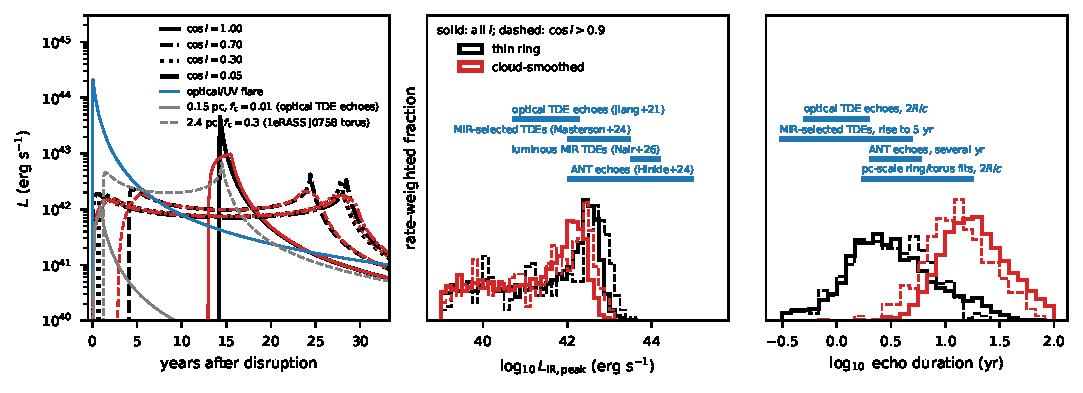
\includegraphics[width=\textwidth]{figures/echo.pdf}
\caption{Left: bolometric light curve of a representative engine disruption (blue; a $b = 0.96$ encounter of a $1~\msun$ star with a $10^{6.0}~\msun$ black hole) and its infrared echo for four inclinations, computed with the transfer function of Equation~(\ref{eq:transfer}) in the thin-ring limit (black) and smoothed over the cloud scale $R_{\rm MC}/c$ (red). Gray curves show the same flare reprocessed by the dust geometries inferred for observed echoes: a $0.15$~pc ring with covering factor $f_c = 0.01$ seen at $45^{\circ}$ (solid; \citealt{vanVelzen:2016a,Jiang:2021b}) and the $2.4$~pc, $f_c = 0.3$ torus at $58^{\circ}$ that \citet{Eyles-Ferris:2026a} fit to 1eRASS~J0758 (dashed). Middle and right: rate-weighted distributions of the peak echo luminosity and of the duration above half maximum for the engine population in the same two limits; solid histograms include all sightlines, dashed ones the unobscured face-on subset with $\cos i > 0.9$, renormalized to the same area. Blue bars mark the ranges measured or inferred for the cited echo samples: the peak dust luminosities of optically selected TDEs \citep{Jiang:2021b}, mid-infrared-selected TDEs \citep[$L_{\rm W2}$;][]{Masterson:2024a}, luminous mid-infrared-selected TDEs \citep{Nair:2026a}, and ambiguous nuclear transients \citep{Hinkle:2024b}; and, for durations, the light-travel spans $2 R_{\rm dust}/c$ of the sub-parsec dust of the first two samples (extended to the five years over which the mid-infrared-selected events remain bright), the several-year echoes of the ambiguous nuclear transients, and the $2R/c$ of the $0.26$--$2.75$~pc rings and tori fitted to individual echoes by \citet{Eyles-Ferris:2026a} and \citet{Wu:2026a}. Bar labels abbreviate these samples.}
\label{fig:echo}
\end{figure*}

The echo calculation overturns the intuition with which we began. Because the engines that dominate the population sit at $10^{6.2}$--$10^{6.7}~\msun$, the inner edge of the disk is at $r_{\rm in} = 3.3$--$11~{\rm pc}$ (16th--84th percentiles, median $5.3$~pc) and the light-travel time $\tau_{0} = r_{\rm in}/c$ has a median of $18$~yr, with a tail to $35$~yr for the engines that have grown toward the ceiling. For an exactly face-on disk the echo is a delayed copy of the flare carrying $\fom = 22\%$ of its luminosity, but the ring spreads the echo over $2 \tau_{0} \sin i$: at $\tau_{0} = 18$~yr an inclination of $3^{\circ}$ spreads it over $1.8$~yr, comparable to the duration of the slowed flares, and $10^{\circ}$ over $6$~yr (Figure~\ref{fig:echo}). Averaged over the $\cos i > 0.9$ sightlines that see the flare unobscured, the peak echo luminosity in the thin-ring limit is $10^{41.7}~{\rm erg~s^{-1}}$ (16th--84th percentiles $10^{39.9}$--$10^{42.7}$) and its duration above half maximum $4$~yr; edge-on sightlines give $10^{41.5}~{\rm erg~s^{-1}}$ over a similar duration, because the ring's transfer function is singular at its two edges. Smoothing over the cloud scale $R_{\rm MC}/c$, which is $2$--$12$~yr across the engine mass range because $R_{\rm MC} \propto \mhsix^{1.49}$, lowers the peak to $10^{41.3}~{\rm erg~s^{-1}}$ and stretches the duration to $13$~yr face-on and $20$~yr edge-on. Because the flares themselves now last a year rather than a month, the echo is less diluted than it would be for prompt flares, but it is also fed by a fainter peak. The inclination dependence is the one \citet{Eyles-Ferris:2026a} and \citet{Tuna:2025a} describe for rings and tori, brighter and shorter toward the pole and fainter and longer toward the plane, with the difference that the engine's ring is so large that only the polar few degrees retain a distinct peak; and since the disruptions in an engine have random orientations relative to the disk, the precession-driven variability of \citet{Wu:2026a} would be superposed on every echo that is resolved in time.

The dust is correspondingly cool. With the echo diluted in time, the equilibrium temperature of \citet{Barvainis:1987a} grains at the echo peak is $190$~K for face-on engines in the thin-ring limit and $160$~K with cloud smoothing, against $37$ and $30$~K for gray grains; the emission peaks at $15$--$30~\um$. This separates the engine echo from the $\sim 10^{42}$--$10^{45}~{\rm erg~s^{-1}}$ echoes at graphite sublimation temperatures that \citet{Hinkle:2024b} find for ambiguous nuclear transients, which arise from dust at sub-parsec radii with comparable covering fractions; the engine's dust is at the same covering fraction but ten times farther out, and it reprocesses at a tenth of the temperature. The consequences for detection are severe in the bands where TDE echoes have been found: a face-on engine echo at $z = 0.01$ has W2 $\simeq 23$ (AB) in the thin-ring limit and $26$ with smoothing, well below the \wise and \spherex limits, and $F213 > 40$ for \romantel. It is, however, bright at $22~\um$: W4 $= 13.8$ (AB; $10.2$ Vega) at $z = 0.01$ and $16.2$ at $z = 0.03$ in the thin-ring limit, $14.6$ and $17.0$ with smoothing, and the same at $21~\um$ for \jwst/MIRI. The AllWISE W4 catalog reaches $\simeq 6$~mJy ($\simeq 14.5$ AB), so an engine echo is detectable in the archival W4 photometry of post-starburst nuclei to $z \simeq 0.015$--$0.02$, and MIRI can follow individual objects to $z \sim 0.1$.

Figure~\ref{fig:echo} places these predictions against the echoes that have been measured. The middle panel marks the peak dust luminosities of the four samples discussed in Section~\ref{subsec:echo}: $10^{40.7}$--$10^{42.3}~{\rm erg~s^{-1}}$ for the optically selected TDEs of \citet{Jiang:2021b}, $10^{42}$--$10^{43.5}$ for the mid-infrared-selected TDEs of \citet{Masterson:2024a}, $10^{43.5}$--$10^{44.2}$ for the luminous events of \citet{Nair:2026a}, and $10^{42}$--$10^{45}$ for the ambiguous nuclear transients of \citet{Hinkle:2024b}. The engine distribution, with its median at $10^{41.3}$--$10^{41.7}~{\rm erg~s^{-1}}$ and its bright tail reaching $10^{42.7}$, overlaps the optically selected echoes and the faint end of the mid-infrared-selected sample and falls short of the rest, even though its covering factor of $0.22$ is twenty times that of the optically selected TDEs and equal to the mean of the ambiguous nuclear transients: the luminosity that the covering factor would buy is spent on the time dilution of a ring ten to fifty times larger. In the right panel the light-travel spans $2 R_{\rm dust}/c$ of the same samples, $0.5$--$2$~yr for the dust within $0.3$~pc of the optically selected TDEs, $0.3$--$5$~yr for the $0.05$--$0.46$~pc shells of \citet{Masterson:2024a} and the five years over which those events stay bright, and the several-year echoes of the ambiguous nuclear transients, all lie below the engine's $4$--$20$~yr; only the parsec-scale rings and tori that \citet{Eyles-Ferris:2026a} and \citet{Wu:2026a} fit to individual echoes, $0.26$--$2.75$~pc with $2R/c = 1.7$--$18$~yr, reach into the engine's range, and their fitted radii, $2.4$~pc for 1eRASS~J0758 and $2.0$~pc for AT~2022agi, are within a factor of two of the engine's inner edge at the floor. The left panel makes the same point for a single flare: reprocessed by the $0.15$~pc, $f_c = 0.01$ shell of the optically selected echoes, the representative flare returns an echo of $10^{41.9}~{\rm erg~s^{-1}}$ that lasts five years, the slowed flare's own duration, and by the $2.4$~pc, $f_c = 0.3$ torus of 1eRASS~J0758 one of $10^{43.0}~{\rm erg~s^{-1}}$ lasting $16$~yr, against the engine ring's $10^{43.3}~{\rm erg~s^{-1}}$ face-on and $10^{42.8}~{\rm erg~s^{-1}}$ at $45^{\circ}$ over $5$ and $23$~yr. The engine echo is therefore not a scaled-up version of the echoes in the literature but a different regime, long and cool, and the objects most like it are the few for which parsec-scale dust has been inferred from the shape of the echo rather than from its temperature.

Because the echo of one disruption lasts a substantial fraction of the $\sim 50$~yr interval to the next at the floor, engines are rarely without one. The fraction of time an engine spends above $10^{41}~{\rm erg~s^{-1}}$ in reprocessed light is $0.09^{+0.33}_{-0.09}$ in the thin-ring limit, and the time-averaged reprocessed luminosity, $\fom \gameq E_{\rm rad}$, is $2.0 \times 10^{41}~{\rm erg~s^{-1}}$; with cloud smoothing the two approach one another and the echo of any single event is barely distinguishable from the steady warm-dust floor. The observable is therefore not an orphan flare but a nuclear $22~\um$ excess of $\sim 10^{41}~{\rm erg~s^{-1}}$ at $T \sim 150$--$200$~K, varying by factors of a few on decade timescales, in a galaxy whose nucleus should otherwise be quiescent; the orphan-echo picture survives only for engines within a few degrees of face-on, which the concentration of the population near the floor, where $\tau_{0} \simeq 11$~yr, makes somewhat less rare than it would be for more massive engines.

\subsection{Model variants}\label{subsec:variants}

Table~\ref{tab:variants} (Appendix~\ref{app:tables}) collects the engine population's summary statistics across the variants of Sections~\ref{subsec:occupation}--\ref{subsec:darkyear}; the numbers that matter are quoted below. The three ingredients that distinguish the fiducial model from the simplest one, a resupplied disk, black holes that grow throughout the post-starburst phase, and slowed circularization, act on different parts of the population, and the table separates them by removing one at a time.

The first two set the rate budget and the mass distribution. Removing the resupply (the gas-limited variant) lowers the active fraction from $21\%$ to $8\%$ and $\dot n_{\rm eng}$ from $3.6$ to $1.0 \times 10^{-8}~{\rm Mpc}^{-3}~{\rm yr}^{-1}$, because $t_{\rm gas}$ at the floor is only $2.7 \times 10^{7}$~yr; it also moves the median engine mass from $10^{6.1}$ to $10^{6.4}~\msun$, since with $t_{\rm gas} \propto \mhsix^{2.33}$ the long-lived engines are the massive ones. Applying the $M_{\rm h}$--$M_\ast$ relation at the burst instead of today (the burst-epoch variant) has a smaller effect on the rate, lowering the active fraction to $17\%$ and raising the required $\fspark \lamc$ from $2.8$ to $4.0$, but it too moves the population off the floor, to a median of $10^{6.2}~\msun$, because more nuclei are then seeded inside the window and fewer arrive at $M_{\rm floor}$ by growth. Removing both (the simple model) compounds the two: the active fraction is $8\%$, $\dot n_{\rm eng} = 8 \times 10^{-9}~{\rm Mpc}^{-3}~{\rm yr}^{-1}$, the required $\fspark \lamc$ is $12$, and the mass distribution is bimodal with a median of $10^{6.47}~\msun$, dominated by engines seeded near the ceiling. The two ingredients reinforce one another because a nucleus that crosses the floor by accretion has its whole lifetime ahead of it only if that lifetime is not cut short by gas exhaustion. The concentration of post-starburst TDEs at the mass floor, which \citet{Guillochon:2026a} took as the engine's signature, is therefore conditional: it requires both that the black holes grow through the phase and that the disk be fed, and a measurement of the black hole masses of post-starburst TDEs constrains the accretion history of their hosts as much as the engine itself.

The third ingredient leaves the rates and masses untouched and changes every light curve. The prompt variant, which draws $T_{\rm visc}$ from the fitted sample, shows what the fiducial population would look like if circularization were fast: engine flares peak $27$~d after first fallback rather than $109$, decline to half maximum in $54$~d rather than $268$, and are brighter by $0.7$~dex at the median ($M_g = -18.3$ against $-16.5$), with $47\%$ of the full disruptions within $10\%$ of the Eddington cap against $19\%$. The partial disruptions, which arrive at low $\beta$ and hence large $r_{\rm p}/r_{\rm g}$, are the events the slowdown affects most: prompt, they are faster than the full disruptions ($43$ against $151$~d) and $0.9$~dex fainter; slowed, they are slower ($300$ against $210$~d) and $1.7$~dex fainter. Their late-time slope steepens from $-1.5$ to $-1.8$ when circularization is prompt, recovering the $t^{-9/4}$ signature that the viscous smoothing erases. The field population, sitting at lower masses, is slowed more severely than the engine: prompt, its median $M_g$ is $-17.5$ and its half-decline time $72$~d, against $-14.9$ and $560$~d slowed, and its \lsst yield is halved by the slowdown where the engine's falls by a third; this is the direction \citet{Guillochon:2015a} proposed as the resolution of the discrepancy between predicted and observed TDE rates, and it raises the engine share of a flux-limited sample at fixed $\fspark \lamc$. The circularization physics therefore does not change what the engine predicts about which black holes are disrupting, but it changes what their flares look like by an order of magnitude in both timescale and luminosity, and it is the ingredient whose observational status is least settled.

\subsection{Survey yields}\label{subsec:yields}

Table~\ref{tab:yields} (Appendix~\ref{app:tables}) lists the number of events per year brighter than an approximate single-epoch threshold in each survey, for the field population rescaled to the observed rate, for the engine population at $\fspark \lamc = 1$, and for the rate-matched engine population. Per unit $\fspark \lamc$ the engine yields $16$~yr$^{-1}$ in ZTF ($g < 19.5$), $370$~yr$^{-1}$ in the \lsst Wide-Fast-Deep survey ($g < 24$), $180$~yr$^{-1}$ in the \romantel High Latitude Wide Area Survey ($F106 < 26$), $0.3$~yr$^{-1}$ in \neowise W1 ($< 19.0$~AB), and $4$~yr$^{-1}$ in the $1.6$--$2.4~\um$ \spherex array ($< 19.5$~AB), and $720$ engine flares are above the \euclid Wide limit ($VIS < 24.5$) in its footprint at any instant; the corresponding field numbers at the observed optical rate are $53$, $1840$, $1290$, $1.3$, $12$, and $3840$. Because engine flares are more luminous than field flares at fixed volumetric rate, the engine share of a flux-limited sample exceeds its share of the volumetric rate: at the rate-matched normalization engines would supply $45\%$ of ZTF's TDEs and $36\%$ of \lsst's, against the third of the optical sample that is actually found in post-starburst hosts. Matching the ZTF detected fraction instead of the volumetric rate gives $\fspark \lamc \simeq 1.7$, consistent with Equation~(\ref{eq:fspark}) within the uncertainty of the post-starburst share itself. \lsst and the \euclid Wide Survey are the surveys in which engine disruptions are numerous, at $\sim 10^{3}$~yr$^{-1}$ at the rate-matched normalization and with median redshifts of $0.6$; the \euclid and \romantel wide surveys visit each field once and will catch engine flares in the act rather than discover them, but their near-infrared depth makes them the only surveys in which the $A_V = 50$ sightlines are recoverable at $z \gtrsim 0.05$. The mid-infrared surveys detect the direct light of a few engine disruptions per year in W1 and the $1.6$--$2.4~\um$ \spherex array, all at $z \lesssim 0.2$, and a few per decade at $4$--$5~\um$. In every survey the detected engine population is drawn from the upper half of the mass window and is one quarter to one third partial disruptions, against $72\%$ intrinsically: the flux limit selects the full disruptions, and the fainter, slower partial majority is what the surveys miss.

\section{Discussion}\label{sec:discussion}

\subsection{What the engine fixes and what it does not}\label{subsec:tests}

The engine hypothesis differs from a generic ``post-starburst nuclei have high rates'' hypothesis in four measurable ways, and the synthetic population shows which of them survive contact with the flare physics we do not understand.

The black hole mass band is the most robust. Its edges follow from $M_{\rm floor}$ and $M_{\rm ceil}$, which are set by the compression and momentum-dominance criteria and do not involve $\lamc$; where within the band the population sits follows from the growth history and the lifetime. In the fiducial model the disruptions in post-starburst hosts are concentrated near the floor, $10^{5.9}$--$10^{6.5}~\msun$ with a median of $10^{6.1}$, because the nuclei that dominate the population are the ones that have just grown across it. Against a field population whose flux-limited masses span $10^{5.3}$--$10^{6.7}~\msun$ in our model, the signature is not so much an offset as a narrowness: a single decade of mass with a hard lower edge. \citet{Shepherd:2026a} find that post-starburst hosts occupy the lower end of the {\it stellar} mass range of the TDE sample and that low-mass hosts carry the late peak of the delay time distribution, and \citet{Ramsden:2026a} find that the quenched TDE hosts in that mass range carry black holes below $10^{6.5}~\msun$, undermassive for their stellar mass; the black hole mass prediction here is for the light curves, and the three are reconciled by the \citet{Reines:2015a} relation, in which $10^{10}~\msun$ hosts carry $10^{6.4}~\msun$ black holes today and carried smaller ones at the burst.

The luminosity of the full disruptions follows from the mass band. Gathered near the Eddington luminosity of a $10^{6}~\msun$ black hole, $10^{43.7}$--$10^{44.35}~{\rm erg~s^{-1}}$, they make the luminous end of the post-starburst TDE luminosity function flat and place it a magnitude brighter than the field's, and their peak luminosity carries little information about $M_\ast$ and $\beta$. The partial fraction of $72\%$ follows from the full loss cone and is the property least sensitive to everything else; it is also the property hardest to measure, since a fitter will return full-disruption solutions for most of these events (Section~\ref{subsec:recovery}) and flux limits remove two thirds of them, and it manifests instead as a faint end populated down to $M_g = -10$ and, for the prompt minority, as late-time slopes steeper than $t^{-5/3}$.

The obscured fraction and its step-function dependence on inclination follow from the disk geometry alone. The echo also follows from geometry, but our calculation shows that the geometry works against detection: the reprocessed light emerges at $\sim 200$~K over years to decades rather than at $\sim 300$~K over a year, and the test moves from \wise W1/W2 and \spherex to W4, MIRI, and the far-infrared. What does {\it not} follow from the engine is anything that depends on $\epsilon$, $R_{\rm ph,0}$, or $l$: the temperatures, the photospheric radii, and the colors are inherited from the fitted sample and are the same for both populations by construction. The viscous time occupies a middle ground: the engine fixes $M_{\rm h}$ and hence $r_{\rm p}/r_{\rm g}$, so if the circularization physics of \citet{Guillochon:2015a} is right the engine also fixes how slowed its flares are.

\subsection{Parameter recovery in the engine regime}\label{subsec:recovery}

The engine's most direct prediction is about the black hole masses of disruptions in post-starburst hosts, and the natural test is to fit the \lsst light curves of such events. \citet{Angus:2026a} show what to expect from that exercise. Fitting simulated \lsst light curves of a well-characterized event with \mosfit, they recover $M_{\rm h}$ with a mean offset of $-0.12$~dex for Deep Drilling Field cadence and $-0.5$~dex for Wide-Fast-Deep cadence, the bias arising from sparse sampling of the rise and the absence of rest-frame near-ultraviolet coverage; a similar tendency appears in the population simulations of \citet{Magill:2026a}. The \lsst-detected engine population sits at $\log M_{\rm h} = 5.9$--$6.5$, and a $0.5$~dex underestimate would place most of its events below $M_{\rm floor}$, where the model forbids them. Three features of the engine population aggravate this. Its full disruptions sit near the Eddington luminosity, so the peak carries little information about the fallback rate and the mass must come from the timescale; its light curves are dominated by partial disruptions, which a fitter constrained to the polytropic grid will interpret as full disruptions of low-mass stars \citep{Angus:2026a}; and, if circularization is slowed as in our fiducial model, the timescale itself measures the viscous time rather than the fallback time, so that a fitter assuming prompt accretion would return masses an order of magnitude too high, in the opposite direction from the cadence bias. A \mosfit fit that leaves $T_{\rm visc}$ free can in principle separate the two, but \citet{Mockler:2019a} found that the optical sample gave no purchase on it, and the degeneracy between $T_{\rm visc}$ and $M_{\rm h}$ in the light-curve width is exactly the one that the engine population, with its narrow mass range and long viscous times, would occupy. The recovered stellar-mass distribution of engine TDEs will therefore not reveal the young population that the engine consumes, and any test of that prediction must come from the hosts' stellar populations \citep{Mockler:2022a} rather than from the flares. The mass test is more tractable: the prediction is for a {\it band} of masses, $7 \times 10^{5}$--$5 \times 10^{6}~\msun$, and a systematic offset of $0.1$--$0.5$~dex shifts the band without erasing it, provided the field population in the same survey is fit with the same pipeline and the comparison is differential. Plateau-luminosity estimators \citep{Mummery:2024a,Mummery:2025a} are free of the full-versus-partial systematic but require late-time UV/optical detections that will be available only at $z \lesssim 0.1$. \citet{Mummery:2026a} offers a middle route: empirical relations between the early optical flare and the black hole mass, calibrated on the plateau and X-ray emission that relativistic disk models describe well, which recover masses for partial and full disruptions alike without late-time data and reproduce the galaxy scaling relations for $89$ events. That calibration is on prompt, optically selected flares, and applying it to a population whose light curves are stretched by slowed circularization would inherit the same timescale ambiguity as a fallback fit; \citet{Mummery:2026a} also emphasize the Malmquist--Hills bias, the joint effect of flux limits and the Hills mass on the recovered mass function, which for the engine population acts to favor the massive end of an already narrow window and is what moves the detected medians of Section~\ref{subsec:rates_result} above the intrinsic one.

\subsection{Relation to the infrared-selected population}\label{subsec:irpop}

The mid-infrared-selected TDEs of \citet{Masterson:2024a}, found as \wise flares of $10^{42}$--$10^{43}~{\rm erg~s^{-1}}$ at $\sim 1000$~K in nearby galaxies, occur at a volumetric rate comparable to the optical one and sit in star-forming, gas-rich hosts rather than post-starburst ones. They are dust echoes of flares hidden at optical wavelengths, and their dust is at the sublimation temperature, hence at $\lesssim 0.1$~pc, with covering fractions of tens of percent; \citet{Hinkle:2024b} find the same covering fractions for the echoes of ambiguous nuclear transients and \citet{Nair:2026a}, extending the \neowise search to luminous events, find that the rate of infrared-selected TDEs above $L_{\rm W2} \simeq 3 \times 10^{43}~{\rm erg~s^{-1}}$ is suppressed to $1.2 \times 10^{-10}~{\rm Mpc}^{-3}~{\rm yr}^{-1}$, a turnover they attribute to the scarcity of the massive black holes needed to power them. The engine's obscured population is different in every one of these respects. Its dust is at $\sim 5$~pc and $\sim 200$~K, so the reprocessed light emerges at $15$--$30~\um$ rather than $3$--$5~\um$ and is not what a W1$-$W2 color selection finds; its hosts are post-starburst by construction; and its reprocessed luminosities, $10^{41}$--$10^{42}~{\rm erg~s^{-1}}$, lie an order of magnitude below the luminous events \citet{Nair:2026a} count. The \citet{Masterson:2024a} population could still be connected to the engine at an earlier stage: \citet{Guillochon:2026a} describe a sparking phase in which the enhanced disruption rate has begun to drive turbulence in the clouds but has not yet suppressed star formation, and a gas-rich, star-forming nucleus with a high covering fraction of hot dust is what that phase would look like from outside. Whether the two populations are related is testable with their hosts: the engine predicts obscured, cool-dust events in post-starburst galaxies specifically, and the fraction of a $20~\um$-selected sample that lands in such hosts, against the near absence of post-starburst hosts among the $3$--$5~\um$-selected events to date, is the discriminant. \citet{Grotova:2025a} find that $30\%$ of their X-ray-selected TDEs show mid-infrared flares and $20\%$ optical ones, in green-valley hosts; an engine seen over its disk would contribute to that X-ray-selected sample with a weak, cool echo rather than a hot one.

\subsection{Caveats}\label{subsec:caveats}

The assumption that the intrinsic flare is independent of environment is the one most likely to fail. The engine nucleus contains an accretion flow at $f_{\rm Edd} \sim 0.05$ and gas at $n \sim 10^{4}~{\rm cm}^{-3}$ within the sphere of influence; the debris stream will interact with both, and the pre-existing disk may alter the circularization efficiency and hence $\epsilon$ and $T_{\rm visc}$ \citep{Chan:2019a}. The compressed cusp also raises the probability that the disrupted star was itself a collision product. We have not modeled any of these.

The three ingredients that separate the fiducial model from the simple one (Section~\ref{subsec:variants}) are the ones we regard as most in need of resolution, and none of them is settled by the engine model itself. Whether the relation of \citet{Reines:2015a} describes post-starburst black holes at the burst or a Gyr later is a question about the accretion history of these nuclei that the engine connects, through Equation~(\ref{eq:ton}), to the delay time distribution of \citet{Shepherd:2026a}; the fiducial reading, in which the black holes grow through the phase, is the one that reproduces the rise to a peak near a Gyr, and it is also the one that populates the mass floor. Whether the circumnuclear disk is fed from the host's larger reservoir is a question about gas transport on tens of parsecs that the resolved molecular disks of nearby Seyferts \citep{GarciaBurillo:2021a} suggest is answered in the affirmative but that post-starburst nuclei have not yet been observed at the required resolution to confirm. Whether circularization is prompt or slowed in the engine window is a question about the debris dynamics that \citet{Guillochon:2015a} showed depends on black hole spin and disk viscosity, neither of which we constrain; its answer determines whether the timescales of engine light curves measure $M_{\rm h}$ at all.

The fallback-following model itself is under pressure. \citet{Mummery:2025b} argue from the observed scaling of radiated energy and peak luminosity with $M_{\rm h}$ that optical light curves do not track the fallback rate, and \citet{Steinberg:2024a} locate the peak light in stream--disk shocks. In the engine regime, where fallback is super-Eddington by one to two orders of magnitude, the \mosfit luminosity is set by the Eddington cap rather than by the fallback rate for most of the flare, and the peak luminosity and its scaling with $M_{\rm h}$ are correspondingly insensitive to which of these pictures is correct; the decline timescale and the late-time slope are not, and the partial-disruption signatures of Section~\ref{subsec:partial} depend on the fallback rate being visible in the light curve at $\gtrsim 200$~d.

The echo calculation treats the inner face of the disk as a smooth, optically thick surface at a single radius, smoothed over the cloud scale, and is a forward model only: fitting the echo of a real event, with the transfer function and dust temperature profile as free parameters alongside the flare, would require a dust-reprocessing module in \mosfit, which we defer to a future paper. The real inner edge is set by $\sim 40$ discrete clouds and the inter-cloud medium, and the echo will be correspondingly lumpy in time. The disk's own thermal emission and the reprocessing of the ambient AGN luminosity provide a background against which the echo must be detected.

Finally, the entire calculation inherits the two-decade normalization uncertainty in $\gameq$ from \citet{Guillochon:2026a}, and the rate budget of Section~\ref{subsec:budget} shows that the fiducial normalization must be raised by a factor of $2$--$3$ to supply the post-starburst TDEs, or by an order of magnitude if the disk is not resupplied. We have framed the population synthesis so that $\fspark \lamc$ is a parameter to be constrained rather than an input to be trusted, and the {\it properties} of the engine population, its mass band, its partial fraction, its obscured fraction, and its echoes, all follow from the equilibrium geometry, which is insensitive to the collision normalization.

\section{Summary}\label{sec:summary}

We have constructed a population model for tidal disruptions in the self-sustaining engine nuclei proposed by \citet{Guillochon:2026a}, combining the engine's mass window, mass-dependent rate, lifetime, and switch-on delay with the local galaxy and black hole mass functions and with black holes that grow through the post-starburst phase, and have generated the light curves of $6000$ engine and $6200$ field disruptions with \mosfit, retaining the partial disruptions that dominate both populations, setting the circularization time from the encounter geometry, and treating the circumnuclear disk as a screen and a reprocessor. The principal results are:
\begin{enumerate}
\item A fifth of post-starburst nuclei host an active engine, and the engine rate density is $3.6 \times 10^{-8}~{\rm Mpc}^{-3}~{\rm yr}^{-1}$ for $\fspark \lamc = 1$. Supplying the post-starburst share of the observed TDE rate requires $\fspark \lamc \simeq 2.8$ by volumetric rate or $\simeq 1.5$ by detected fraction, within a factor of a few of the fiducial normalization. The budget depends on the disk being resupplied and on the black holes growing throughout the phase: an isolated disk lowers the active fraction to $8\%$ and raises the requirement to $\fspark \lamc \simeq 10$.
\item The black hole mass distribution of engine disruptions is concentrated near the floor, $10^{5.9}$--$10^{6.5}~\msun$ with a median of $10^{6.1}~\msun$, because the population is dominated by nuclei that have just grown across $M_{\rm floor}$. The signature is a single decade of mass with a lower edge as sharp as the nucleus-to-nucleus scatter in the floor allows ($\sim 0.1$~dex); flux limits move the detected subsets to $10^{6.16}$ (\lsst) and $10^{6.4}~\msun$ (ZTF), $0.2$--$0.45$~dex above the field's.
\item $72\%$ of engine disruptions are partial, against $67\%$ in the field, and the fraction is set by the loss-cone regime rather than by the age of the disrupted stars. The full disruptions gather near the Eddington luminosity of a $10^{6}~\msun$ black hole, $L_{\rm peak} = 10^{43.7}$--$10^{44.35}~{\rm erg~s^{-1}}$ and $M_g \simeq -20$; the partial disruptions are $1.7$~dex fainter at the median and extend the luminosity function to $M_g = -10$. At the observed optical rate the engine supplies three fifths of the TDEs brighter than $M_g = -20$ while carrying a third of the total.
\item With circularization slowed as \citet{Guillochon:2015a} argue for black holes below $10^{7}~\msun$, engine flares peak $\sim 110$~d after first fallback and decline to half maximum in $\sim 280$~d, several times slower than prompt flares of the same black holes; field flares of smaller black holes are slowed further, to $\sim 560$~d. Partial disruptions, arriving at large $r_{\rm p}/r_{\rm g}$, are slowed most, and the $t^{-9/4}$ decline that identifies them survives only in the prompt minority.
\item A fraction $\fom = 0.22$ of engine disruptions is obscured, as a step function of inclination; the obscured events are recoverable in W1 if the sightline crosses only the inter-cloud medium ($A_V = 50$, $3.7$~mag) and lost if it crosses a cloud ($A_V = 400$).
\item The dust echo is not an orphan mid-infrared flare. With $r_{\rm in}/c \simeq 18$~yr, inclinations above a few degrees spread the reprocessed $22\%$ of the flare energy over years to decades, producing a $10^{41}$--$10^{42}~{\rm erg~s^{-1}}$, $150$--$200$~K component that peaks at $15$--$30~\um$, is invisible to \wise W1/W2 and \spherex, and is detectable in \wise W4 to $z \simeq 0.02$ and with \jwst/MIRI to $z \sim 0.1$. Engines should show a persistent $22~\um$ nuclear excess of $\sim 10^{41}~{\rm erg~s^{-1}}$.
\item At the rate-matched normalization \lsst would detect $\sim 1000$ engine disruptions per year at a median redshift of $0.6$ and \euclid Wide would hold $\sim 2000$ above its single-epoch limit at any time; ZTF detects $16$~yr$^{-1}$ per unit $\fspark \lamc$. Fitting these light curves will recover the mass band only if the viscous delay is modeled, since slowed flares mimic more massive black holes, and the $0.1$--$0.5$~dex cadence bias of \citet{Angus:2026a} acts in the opposite direction; the stellar masses and the partial fraction will not be recovered.
\end{enumerate}

\begin{acknowledgments}
The manuscript source, the bibliography, and the population synthesis and light-curve scripts are available online.\footnote{\url{https://github.com/guillochon/engine-lc}} The authors take full responsibility for the contents of this paper. Large language models (Claude Fable 5.1, Grok 4.6, and GPT5.6 Sol) were used in drafting the text and in deriving and checking the analytic results; every displayed equation has been re-derived independently and every entry in the bibliography was validated against the NASA Astrophysics Data System. This use complies with the AAS policy that such tools are not authors and that responsibility for accuracy remains with the listed authors \citep{Vishniac2025}. We thank J. Xavier Prochaska for providing access to AI models that were used to conduct independent AI reviews. All references and AI edits were hand-checked by the authors.
\end{acknowledgments}

\software{\mosfit \citep{Guillochon:2018a}, {\tt dynesty} \citep{Speagle:2020a}, {\tt astropy} \citep{Astropy:2013a,Astropy:2018a,Astropy:2022a}, {\tt extinction} \citep{Barbary:2016a}, {\tt numpy} \citep{Harris:2020a}, {\tt scipy} \citep{Virtanen:2020a}, {\tt matplotlib} \citep{Hunter:2007a}}

\bibliographystyle{aasjournalv7}
\bibliography{engine-lc}

\appendix

\section{Population, light-curve, variant, and yield tables}\label{app:tables}

The tables referenced in the text are collected here. Table~\ref{tab:params} lists the Monte Carlo distributions of Section~\ref{subsec:params}; Table~\ref{tab:lcstats} the light-curve statistics of the fiducial populations (Section~\ref{subsec:lcdist}); Table~\ref{tab:variants} the engine population across the model variants (Section~\ref{subsec:variants}); and Table~\ref{tab:yields} the survey yields (Section~\ref{subsec:yields}).

\begin{longrotatetable}
\begin{deluxetable}{llll}
\tablecaption{Monte Carlo parameter distributions \label{tab:params}}
\tablehead{\colhead{Parameter} & \colhead{Field population} & \colhead{Engine population} & \colhead{Source}}
\startdata
$M_{\rm h}$ & BHMF $\times\, \Gamma_{\rm field}$, & BHMF $\times f_{\rm eng} \gameq$, growing at $f_{\rm Edd} = 0.05$, & Sections~\ref{subsec:hosts}--\ref{subsec:rates} \\
 & $M_{\rm h} \geq 10^{5}~\msun$ & $M_{\rm floor} < M_{\rm h} < M_{\rm ceil}$ & \\
\noalign{\vskip 1.5pt}\hline\noalign{\vskip 1.5pt}
$M_{\ast}$ & PDMF at 10 Gyr & $\tfrac{1}{2}$ PDMF at burst age & \citet{Kochanek:2016a} \\
 & $\times$ tidal cross-section & $+ \tfrac{1}{2}$ PDMF at 10 Gyr & \\
\noalign{\vskip 1.5pt}\hline\noalign{\vskip 1.5pt}
$\beta$ & $\beta^{-2}$ (pinhole fraction $0.6 \to 0.1$) & $\beta^{-2}$ ($70\%$) $+$ grazing ($30\%$) & \citet{Stone:2016a}; \\
 & $+$ grazing & & \citet{Guillochon:2026a} \\
\noalign{\vskip 1.5pt}\hline\noalign{\vskip 1.5pt}
$\epsilon$, $R_{\rm ph,0}$, $l$ & joint draws from 21 fitted events & same & \citet{Nicholl:2022a} \\
\noalign{\vskip 1.5pt}\hline\noalign{\vskip 1.5pt}
$T_{\rm visc}$ & set by $r_{\rm p}/r_{\rm g}$ (dark year) & same & \citet{Guillochon:2015a}; \\
 & & & Section~\ref{subsec:darkyear} \\
\noalign{\vskip 1.5pt}\hline\noalign{\vskip 1.5pt}
$N_{\rm H,host}$ & fit to optical sample & host $+$ screen($i$) & \citet{Nicholl:2022a}; \\
 & & & Section~\ref{subsec:screen} \\
\noalign{\vskip 1.5pt}\hline\noalign{\vskip 1.5pt}
Dust covering factor & $\sim 0.01$ at $0.1$--$1$~pc & $\fom = 0.22$ at $r_{\rm in}$ & \citet{Jiang:2021b}; \\
 & & & Table~\ref{tab:engine} \\
\noalign{\vskip 1.5pt}\hline\noalign{\vskip 1.5pt}
Inclination $i$ & \nodata & isotropic & \\
\noalign{\vskip 1.5pt}\hline\noalign{\vskip 1.5pt}
Redshift & uniform in comoving volume, $z < 1$ & same & \\
\enddata
\end{deluxetable}
\end{longrotatetable}

\begin{longrotatetable}
\begin{deluxetable}{lcccccc}
\tablecaption{Light-curve statistics of the fiducial populations \label{tab:lcstats}}
\tablehead{\colhead{Quantity} & \colhead{Engine, all} & \colhead{Engine, full} & \colhead{Engine, partial} & \colhead{Field, all} & \colhead{Field, full} & \colhead{Field, partial}}
\startdata
$\log M_{\rm h}/\msun$ & $6.12^{+0.35}_{-0.22}$ & \nodata & \nodata & $5.43^{+0.67}_{-0.32}$ & \nodata & \nodata \\
$M_\ast/\msun$ & $0.35^{+0.42}_{-0.20}$ & \nodata & \nodata & $0.32^{+0.32}_{-0.17}$ & \nodata & \nodata \\
partial fraction & $0.71$ & \nodata & \nodata & $0.66$ & \nodata & \nodata \\
$\log L_{\rm peak}$ (erg s$^{-1}$) & $43.41^{+0.57}_{-1.30}$ & $43.95^{+0.21}_{-0.20}$ & $42.98^{+0.71}_{-1.15}$ & $43.11^{+0.42}_{-0.95}$ & $43.39^{+0.37}_{-0.20}$ & $42.66^{+0.61}_{-0.74}$ \\
fraction with $L_{\rm peak} > 0.9\,L_{\rm Edd}$ & $0.01$ & $0.02$ & \nodata & $0.11$ & $0.30$ & \nodata \\
$M_g$ at peak & $-17.3^{+4.9}_{-2.3}$ & \nodata & \nodata & $-16.6^{+3.8}_{-1.9}$ & \nodata & \nodata \\
$t_{\rm peak}$ after first fallback (d) & $25^{+14}_{-7}$ & \nodata & \nodata & $11^{+13}_{-4}$ & \nodata & \nodata \\
$t_{1/2,\rm decline}$, bolometric (d) & $53^{+28}_{-16}$ & $68^{+29}_{-22}$ & $48^{+23}_{-13}$ & $38^{+29}_{-16}$ & $47^{+26}_{-17}$ & $33^{+28}_{-13}$ \\
$t_{1/2,\rm decline}$, $g$ band (d) & $35^{+33}_{-14}$ & $41^{+27}_{-18}$ & $32^{+35}_{-12}$ & $24^{+28}_{-12}$ & $29^{+22}_{-13}$ & $20^{+31}_{-10}$ \\
${\rm d}\ln L/{\rm d}\ln t$ (200--600 d) & $-1.61^{+0.77}_{-0.26}$ & $-0.88^{+0.26}_{-0.28}$ & $-1.76^{+0.25}_{-0.14}$ & $-1.54^{+1.00}_{-0.30}$ & $-0.61^{+0.19}_{-0.25}$ & $-1.74^{+0.48}_{-0.14}$ \\
$T_{\rm bb}$, constant-$T$ fit ($10^{4}$~K) & $2.8^{+2.4}_{-1.2}$ & \nodata & \nodata & $2.5^{+2.2}_{-1.0}$ & \nodata & \nodata \\
$T_{\rm ph}$ at peak, model ($10^{4}$~K) & $3.1^{+4.7}_{-1.6}$ & \nodata & \nodata & $2.8^{+3.8}_{-1.3}$ & \nodata & \nodata \\
$\log E_{\rm rad}$ (erg) & $50.5^{+1.0}_{-1.4}$ & \nodata & \nodata & $50.1^{+0.8}_{-1.2}$ & \nodata & \nodata \\

\enddata
\tablecomments{Medians with 16th and 84th percentiles, weighted by rate. Generated by {\tt scripts/postprocess.py} from {\tt products/results\_fiducial.json}.}
\end{deluxetable}
\end{longrotatetable}

\begin{longrotatetable}
\begin{deluxetable}{lcccccccccc}
\tablecaption{Engine population across model variants \label{tab:variants}}
\tablehead{\colhead{Variant} & \colhead{$\dot n_{\rm eng}$} & \colhead{$f_{\rm active}$} & \colhead{$\fspark\lamc$} & \colhead{$\log M_{\rm h}$} & \colhead{partial} & \colhead{$\log L_{\rm peak}$} & \colhead{$t_{1/2}$, bol.} & \colhead{$M_g$} & \colhead{ZTF} & \colhead{\lsst} \\
\colhead{} & \colhead{($10^{-9}$ Mpc$^{-3}$ yr$^{-1}$)} & \colhead{} & \colhead{needed} & \colhead{median} & \colhead{fraction} & \colhead{full, median} & \colhead{(d)} & \colhead{median} & \colhead{yr$^{-1}$} & \colhead{yr$^{-1}$}}
\startdata
Fiducial (prompt, fed disk, growing black holes) & 36.2 & 0.210 & 2.8 & 6.12 & 0.71 & 43.95 & 53 & -17.3 & 9.1 & 389 \\
Slowed circularization (dark-year viscous delay) & 36.2 & 0.210 & 2.8 & 6.12 & 0.71 & 43.92 & 103 & -16.3 & 7.7 & 338 \\
Gas-limited lifetime ($\tau = t_{\rm gas}$) & 10.5 & 0.085 & 9.6 & 6.37 & 0.72 & 44.01 & 60 & -17.3 & 3.2 & 117 \\
Relation applies at the burst & 25.1 & 0.171 & 4.0 & 6.22 & 0.71 & 43.98 & 56 & -17.3 & 7.1 & 275 \\
Simple (all three of the above) & 8.2 & 0.079 & 12.2 & 6.47 & 0.74 & 44.10 & 65 & -17.3 & 2.5 & 92 \\
Burst population only & 36.2 & 0.210 & 2.8 & 6.12 & 0.72 & 43.95 & 52 & -17.2 & 8.8 & 390 \\
Old population only & 36.4 & 0.212 & 2.7 & 6.12 & 0.70 & 43.93 & 53 & -17.3 & 6.2 & 392 \\
\citet{Kormendy:2013a} relation & 4.2 & 0.043 & 23.7 & 6.45 & 0.74 & 44.08 & 65 & -17.3 & 1.5 & 49 \\
\citet{Miller:2015a} occupation fraction & 33.8 & 0.199 & 3.0 & 6.13 & 0.70 & 43.94 & 53 & -17.4 & 7.3 & 368 \\
Disk cap at $L_{\rm Edd}$ (no EUV fraction) & 36.2 & 0.210 & 2.8 & 6.12 & 0.71 & 44.33 & 49 & -19.1 & 42.2 & 611 \\
Disk cap at $0.3\,L_{\rm Edd}$ & 36.2 & 0.210 & 2.8 & 6.12 & 0.71 & 44.09 & 56 & -18.1 & 17.6 & 501 \\

\enddata
\tablecomments{$\dot n_{\rm eng}$ and yields are for $\fspark \lamc = 1$; $\fspark\lamc$ needed is the value that supplies $\dot n_{\rm PSB} = 10^{-7}$~Mpc$^{-3}$~yr$^{-1}$. Yields are counted above the thresholds of Table~\ref{tab:yields} with the disk screen at $A_V = 50$. Generated by {\tt scripts/variant\_table.py}.}
\end{deluxetable}
\end{longrotatetable}

\begin{longrotatetable}
\begin{deluxetable}{lcccccc}
\tablecaption{Detection yields per year \label{tab:yields}}
\tablehead{\colhead{Survey (threshold)} & \colhead{Field} & \colhead{Engine, $\fspark\lamc = 1$} & \colhead{Engine, rate-matched} & \colhead{Engine $z_{\rm med}$} & \colhead{Engine $\log M_{\rm h}$} & \colhead{Engine partial fraction}}
\startdata
ZTF ($g < 19.5$) & 27 & 9.1 & 25 & 0.16 & 6.0--6.6 & 0.28 \\
Rubin WFD ($g < 24.0$) & 2403 & 389 & 1076 & 0.62 & 5.9--6.5 & 0.37 \\
Euclid Wide (VIS $< 24.5$) & 887 & 250 & 692 & 0.65 & 5.9--6.5 & 0.40 \\
Roman HLWAS (F106 $< 26.0$) & 284 & 67 & 186 & 0.69 & 5.9--6.5 & 0.49 \\
Roman HLTDS (F106 $< 26.0$) & 5.6 & 0.61 & 1.7 & 0.69 & 5.9--6.5 & 0.49 \\
NEOWISE (W1 $< 19.0$) & 0.00 & 0.16 & 0.45 & \nodata & \nodata & \nodata \\
NEOWISE (W2 $< 18.5$) & 0.00 & 0.00 & 0.00 & \nodata & \nodata & \nodata \\
SPHEREx (S3 $< 19.5$) & 5.1 & 1.1 & 3.2 & 0.12 & 5.9--6.6 & 0.29 \\
SPHEREx (S6 $< 18.5$) & 0.00 & 0.00 & 0.00 & \nodata & \nodata & \nodata \\

\enddata
\tablecomments{Yields are events per year whose peak apparent magnitude exceeds the stated threshold, over the stated sky fraction, with the disk screen at $\Av = 50$. For \euclid Wide and the \romantel High Latitude Wide Area Survey, which visit each field once, the entry is instead the number of events brighter than the threshold in the footprint at any instant. Detection thresholds are approximate single-epoch depths and do not include host-galaxy contamination or cadence.}
\end{deluxetable}
\end{longrotatetable}

\end{document}
